
\documentclass[
% -- opções da classe memoir --
12pt,				% tamanho da fonte
openright,			% capítulos começam em pág ímpar (insere página vazia caso preciso)
oneside,			% para impressão em recto e verso. Oposto a oneside
a4paper,			% tamanho do papel. 
% -- opções da classe abntex2 --
chapter=TITLE,		% títulos de capítulos convertidos em letras maiúsculas
section=TITLE,		% títulos de seções convertidos em letras maiúsculas
%subsection=TITLE,	% títulos de subseções convertidos em letras maiúsculas
%subsubsection=TITLE,% títulos de subsubseções convertidos em letras maiúsculas
% -- opções do pacote babel --
english,			% idioma adicional para hifenização
french,				% idioma adicional para hifenização
spanish,			% idioma adicional para hifenização
brazil				% o último idioma é o principal do documento
]{abntex2-uepg}

% ---
% Pacotes básicos 
% ---
\usepackage{lmodern}			% Usa a fonte Latin Modern			
\usepackage[T1]{fontenc}		% Selecao de codigos de fonte.
\usepackage[utf8]{inputenc}		% Codificacao do documento (conversão automática dos acentos)
\usepackage{indentfirst}		% Indenta o primeiro parágrafo de cada seção.
\usepackage{color}				% Controle das cores
\usepackage{graphicx}			% Inclusão de gráficos
			% para melhorias de justificação]
\usepackage{uepg}
\usepackage{lipsum}		
\usepackage{amssymb}
\usepackage{amsmath}
%\usepackage{paralist}
\usepackage{setspace}
\usepackage{lscape}
\usepackage{longtable}	
\usepackage{listings}
\usepackage{gantt}
\usepackage{inconsolata}
\usepackage{xcolor}
\usepackage[bottom=2cm,top=3cm,left=3cm,right=2cm]{geometry}
\usepackage{titlesec}
\usepackage{caption}
\usepackage{pdfpages}   % inclusão da ficha clínica da LORD (Anexo A)
\usepackage{tabularx}   % quadros com colunas de largura automática
\usepackage{tikz}       % diagramas (estados, contêineres, sequência e DER)
\usetikzlibrary{positioning,arrows.meta,shapes.multipart,shapes.geometric,fit,calc,backgrounds}
\usepackage{multirow}
\captionsetup[table]{
	singlelinecheck=false, % Alinha o caption à esquerda
}
\captionsetup[quadro]{
	singlelinecheck=false, % Alinha o caption à esquerda
}
\captionsetup[figure]{
	singlelinecheck=false, % Alinha o caption à esquerda
}
\titlespacing*{\subsection}{0pt}{2.5ex plus 1ex minus .2ex}{2.5ex plus .2ex} 

\setlength\afterchapskip{\lineskip}

\definecolor{codegreen}{rgb}{0,0.6,0}
\definecolor{codegray}{rgb}{0.5,0.5,0.5}
\definecolor{codepurple}{rgb}{0.58,0,0.82}
\definecolor{backcolour}{rgb}{0.95,0.95,0.92}

\lstdefinestyle{mystyle}{
	backgroundcolor=\color{backcolour},   
	commentstyle=\color{codegreen},
	keywordstyle=\color{magenta},
	numberstyle=\tiny\color{codegray},
	stringstyle=\color{codepurple},
	basicstyle=\ttfamily\footnotesize,
	breakatwhitespace=false,         
	breaklines=true,                 
%	captionpos=b,                    
	keepspaces=true,                 
	numbers=left,                    
	numbersep=5pt,                  
	showspaces=false,                
	showstringspaces=false,
	showtabs=false,                  
	tabsize=2,
	frame=single,
	% listings não trata UTF-8 multibyte no pdflatex: mapeia os acentos do português
	literate={á}{{\'a}}1 {à}{{\`a}}1 {â}{{\^a}}1 {ã}{{\~a}}1 {é}{{\'e}}1 {ê}{{\^e}}1
	         {í}{{\'i}}1 {ó}{{\'o}}1 {ô}{{\^o}}1 {õ}{{\~o}}1 {ú}{{\'u}}1 {ç}{{\c{c}}}1
	         {Á}{{\'A}}1 {É}{{\'E}}1 {Í}{{\'I}}1 {Ó}{{\'O}}1 {Ú}{{\'U}}1 {Ç}{{\c{C}}}1
}

\lstset{style=mystyle}

% Marcador de pendências do texto (aparece em vermelho no PDF).
% Antes da entrega final, procure por "\todo" e remova todas as ocorrências.
\newcommand{\todo}[1]{\textcolor{red}{[\textbf{TODO:} #1]}}

% Colunas alinhadas à esquerda para quadros (evita espaços largos em colunas estreitas)
\newcolumntype{L}[1]{>{\raggedright\arraybackslash}p{#1}}
\newcolumntype{Y}{>{\raggedright\arraybackslash}X}
% espaço vertical nas células: sem ele, as linhas horizontais encostavam no texto das tabelas e quadros
\setlength{\extrarowheight}{3pt}
\renewcommand{\arraystretch}{1.15}

% Nomes usados pelo \autoref para floats personalizados
\providecommand{\quadroautorefname}{Quadro}
\providecommand{\lstlistingautorefname}{Código}

% Espaço reservado para figuras ainda não produzidas
\newcommand{\figtodo}[1]{\fbox{\parbox[c][5cm][c]{0.9\textwidth}{\centering\textcolor{red}{[FIGURA: #1]}}}}

\usepackage[brazilian,hyperpageref]{backref}	 % Paginas com as citações na bibl
\usepackage[alf,
abnt-emphasize = bf, % destaca o titulo da revista ou livro em negrito;
abnt-etal-list = 3, % trabalhos com mais de 3 autores recebem et al.,;
abnt-etal-text = it, % escreve o et al., em italico;
abnt-and-type = &, % usa o carater '&' no lugar de 'e' para mais de um autor;
abnt-last-names = abnt, % trata sobrenomes 'estritamente' conforme a ABNT; e
abnt-repeated-author-omit = no] {abntex2cite}

% ---
% Configurações do pacote backref
% Usado sem a opção hyperpageref de backref
\renewcommand{\backrefpagesname}{Citado na(s) página(s):~}
% Texto padrão antes do número das páginas
\renewcommand{\backref}{}
% Define os textos da citação
\renewcommand*{\backrefalt}[4]{
	\ifcase #1 %
	Nenhuma citação no texto.%
	\or
	Citado na página #2.%
	\else
	Citado #1 vezes nas páginas #2.%
	\fi}%
% ---
% -- ljsenger
\renewcommand{\rmdefault}{phv} % Arial
\renewcommand{\sfdefault}{phv} % Arial

% formatacao de codigo fonte
\renewcommand{\lstlistingname}{Código}
\renewcommand{\lstlistlistingname}{Lista de códigos}

% ---
% Informações de dados para CAPA e FOLHA DE ROSTO
% ---
% Título aprovado na versão preliminar. Sugestão (depende de aval da coordenação):
% Sistema web de prontuário odontológico com anamnese estruturada por
% inteligência artificial e análise da evolução clínica em DTM
\titulo{Desenvolvimento de um sistema web de prontuários eletrônicos com análise de dados de evolução clínica}
% \titulo{Formatação de trabalhos para a UEPG com o uso da classe \abnTeX}
\autor{Gabriel Henrique Pereira Guimarães\\Bruno Cheres de Oliveira Cruz}
 
\local{Ponta Grossa}

\data{2026}

\orientador{Orientador: Prof. Márcio Augusto de Souza}

\coorientador{}


	
\tipotrabalho{Trabalho de Conclusão de Curso}
% O preambulo deve conter o tipo do trabalho, o objetivo, 
% o nome da instituição e a área de concentração 
\preambulo{Trabalho de conclusão de Curso apresentado como requisito parcial para obtenção do
	título de Bacharel em Engenharia de Computação na Universidade Estadual de Ponta Grossa}

\definecolor{blue}{RGB}{41,5,195}

\makeatletter
\hypersetup{
	%pagebackref=true,
	pdftitle={\@title}, 
	pdfauthor={Gabriel Henrique Pereira Guimarães; Bruno Cheres de Oliveira Cruz},
	pdfsubject={\imprimirpreambulo},
	pdfcreator={LaTeX with abnTeX2},
	pdfkeywords={prontuário eletrônico}{odontologia}{DTM}{LGPD}{inteligência artificial}, 
	colorlinks=true,       		% false: boxed links; true: colored links
	linkcolor=black,          	% color of internal links
	citecolor=black,        		% color of links to bibliography
	filecolor=magenta,      		% color of file links
	urlcolor=black,
	bookmarksdepth=4
}
\makeatother
% --- 

% ---
% Posiciona figuras e tabelas no topo da página quando adicionadas sozinhas
% em um página em branco. Ver https://github.com/abntex/abntex2/issues/170
\makeatletter
\setlength{\@fptop}{5pt} % Set distance from top of page to first float
\makeatother
% ---

% ---
% Possibilita criação de Quadros e Lista de quadros.
% Ver https://github.com/abntex/abntex2/issues/176
%
\newcommand{\quadroname}{Quadro}
\newcommand{\listofquadrosname}{Lista de quadros}

\newfloat[chapter]{quadro}{loq}{\quadroname}
\newlistof{listofquadros}{loq}{\listofquadrosname}
\newlistentry{quadro}{loq}{0}


% configurações para atender às regras da ABNT
\setfloatadjustment{quadro}{\centering}
\counterwithout{quadro}{chapter}
\renewcommand{\cftquadroname}{\quadroname\space} 
\renewcommand*{\cftquadroaftersnum}{\hfill--\hfill}

\setfloatlocations{quadro}{hbtp} % Ver https://github.com/abntex/abntex2/issues/176
% ---

% --- 
% Espaçamentos entre linhas e parágrafos 
% --- 

% O tamanho do parágrafo é dado por:
\setlength{\parindent}{1.3cm}

% Controle do espaçamento entre um parágrafo e outro:
\setlength{\parskip}{0.2cm}  % tente também \onelineskip

%ljsenger - espaçamento simples (e feio) entre parágrafos
\setlength{\parskip}{0cm}
%ljsenger - espaçamento entre o título e o primeiro parágrafo do texto
\setlength\afterchapskip{18pt}

% compila o indice
\makeindex
% ---
% padrão UEPG - fonte ARIAL (ou times)
\renewcommand{\rmdefault}{phv} % Arial
\renewcommand{\sfdefault}{phv} % Arial

\newlistof{lstlistoflistings}{lol}{\lstlistlistingname}
\begin{document}
	
	\selectlanguage{brazil}
	\frenchspacing 
	
	\imprimircapa
	% ---
	
	% ---
	% Folha de rosto
	% (o * indica que haverá a ficha bibliográfica)
	% ---
	\imprimirfolhaderosto
	
	% Elementos opcionais: descomente quando estiverem escritos
	%% ---
% Dedicatória (opcional). Para usar, descomente % ---
% Dedicatória (opcional). Para usar, descomente % ---
% Dedicatória (opcional). Para usar, descomente \input{dedicatoria} no tcc.tex
% e escreva o texto abaixo; se não houver dedicatória, deixe o \input comentado.
% ---
\begin{dedicatoria}
	\vspace*{\fill}
	\centering
	\noindent
	\textit{(texto da dedicatória)}
	\vspace*{\fill}
\end{dedicatoria}
 no tcc.tex
% e escreva o texto abaixo; se não houver dedicatória, deixe o \input comentado.
% ---
\begin{dedicatoria}
	\vspace*{\fill}
	\centering
	\noindent
	\textit{(texto da dedicatória)}
	\vspace*{\fill}
\end{dedicatoria}
 no tcc.tex
% e escreva o texto abaixo; se não houver dedicatória, deixe o \input comentado.
% ---
\begin{dedicatoria}
	\vspace*{\fill}
	\centering
	\noindent
	\textit{(texto da dedicatória)}
	\vspace*{\fill}
\end{dedicatoria}

	\begin{agradecimentos}
		% Agradecimentos (opcional). Para usar, descomente o bloco correspondente no tcc.tex.
% Rascunho: ajuste os nomes e acrescente os agradecimentos pessoais.

Ao Prof. Márcio Augusto de Souza, pela orientação, pela disponibilidade e pelas críticas que deram forma a este trabalho.

Aos membros e professores da Liga Odontológica de Reabilitação e DTM (LORD-UEPG), que apresentaram o problema, explicaram a rotina da clínica e a ficha clínica e confiaram a nós a sua digitalização.

Aos professores do Departamento de Informática (DEINFO) da UEPG, pela formação ao longo do curso, e aos membros da banca de qualificação, cujos pareceres melhoraram a proposta.

Às nossas famílias e amigos, pelo apoio durante a graduação.

	\end{agradecimentos}
	% ---
	
	% ---
	% Epígrafe
	% ---
	\begin{epigrafe}
	\vspace*{\fill}
	\begin{flushright}
		\textit{``Conheça todas as teorias, domine todas as técnicas,\\ mas ao tocar uma alma humana,\\ seja apenas outra alma humana.''\\ (Carl Jung)}
	\end{flushright}
\end{epigrafe}

	\setlength{\absparsep}{18pt} % ajusta o espaçamento dos parágrafos do resumo
	\begin{resumo}
		Este trabalho apresenta o desenvolvimento de um sistema web de prontuários eletrônicos para a Liga Odontológica de Reabilitação e DTM da Universidade Estadual de Ponta Grossa (LORD-UEPG). A motivação decorre da gestão inadequada de prontuários físicos em tratamentos contínuos, como os de disfunção temporomandibular (DTM) e de reabilitação protética, que resulta na perda de informações essenciais ao acompanhamento longitudinal. O sistema digitaliza a ficha clínica da Liga a partir de um esquema de dados versionado, persistido em modelo híbrido relacional e documental (PostgreSQL com JSONB), com controle de acesso por papéis, fluxo de supervisão docente, trilha de auditoria e pseudonimização dos dados destinados à pesquisa, em conformidade com a Lei Geral de Proteção de Dados. Como diferencial, o sistema incorpora um módulo de inteligência artificial executado localmente, que transcreve a fala do acadêmico e estrutura as informações narrativas da anamnese nos campos da ficha, sem emitir diagnóstico: toda sugestão é revisada e aprovada por um humano. Um módulo analítico em Python calcula indicadores de evolução clínica, como as escalas de dor, a Escala Graduada de Dor Crônica do RDC/TMD e a amplitude de abertura bucal. A avaliação compreendeu a qualidade da estruturação automática em casos clínicos sintéticos, a comparação entre entrada por áudio e por texto, um teste de usabilidade com membros da Liga e a validação do pipeline analítico com uma coorte sintética de efeito conhecido. \todo{inserir os principais resultados numéricos: F1 da extração, taxa de alucinação, WER, escore SUS e tempo de preenchimento em relação ao papel.}

\textbf{Palavras-chave}: Prontuário eletrônico. Odontologia. Disfunção temporomandibular. Inteligência artificial. Proteção de dados.

	\end{resumo}
	
	% resumo em inglês
	\begin{resumo}[Abstract]
		\begin{otherlanguage*}{english}
			This work presents the development of a web-based electronic health record system for the Dental Rehabilitation and TMD Academic League of the State University of Ponta Grossa (LORD-UEPG). The motivation lies in the limitations of paper records in the follow-up of long-term treatments, such as those for temporomandibular disorders (TMD) and prosthetic rehabilitation, in which the information recorded at each visit must be compared over time. The system digitizes the League's clinical form from a versioned description of the form, stored in a database that combines tables and documents (PostgreSQL with JSONB), with role-based access control, faculty supervision workflow, audit trail and pseudonymization of research data, in compliance with the Brazilian General Data Protection Law. It includes a locally executed artificial intelligence module that transcribes the student's speech and organizes the anamnesis report into the form fields without issuing any diagnosis: each suggestion is reviewed individually by a human. An analytical module in Python computes clinical progress indicators, such as pain scales, the RDC/TMD Graded Chronic Pain Scale and mouth opening. On 30 synthetic clinical cases, the local 3-billion-parameter language model reached an F1 score of 0.59, and automatic checks of the suggestions reduced from 32\% to 25\% the proportion of empty fields wrongly filled, which confirms the need for human review. Speech transcription, using a synthetic voice, missed about 4\% of the words in silence and 6\% with simulated noise, with errors concentrated in clinical terms. With 10,000 patients, the hybrid model read a patient record three to four times faster than a fully relational model and used almost half the storage. The usability evaluation, carried out without participants, found no accessibility violations in the main screens and estimated about 9.7 minutes to fill in the complete form. On a synthetic cohort with known effects, the analytical module recovered the pain reductions programmed for the three treatments. The results indicate that it is feasible to keep the data within the institution using free tools and to use AI only to support clinical documentation.
			
			\vspace{\onelineskip}
			
			\noindent 
			\textbf{Keywords}: Electronic health records. Dentistry. Temporomandibular disorders. Artificial intelligence. Data protection.
		\end{otherlanguage*}
	\end{resumo}
	
	% inserir lista de ilustrações
	% ---
	\renewcommand{\listfigurename}{Lista de figuras}
	\pdfbookmark[0]{\listfigurename}{lof}
	\listoffigures*
	\cleardoublepage
	% inserir lista de quadros
	% ---
	\pdfbookmark[0]{\listofquadrosname}{loq}
	\listofquadros*
	\cleardoublepage
	% inserir lista de tabelas
	% ---
	\pdfbookmark[0]{\listtablename}{lot}
	\listoftables*
	\cleardoublepage
	% inserir lista de abreviaturas e siglas
	% ---
	%\pdfbookmark[0]{\lstlistlistingname}{lot}
	\lstlistoflistings*
	\cleardoublepage
	% inserir lista de abreviaturas e siglas
	\begin{siglas}
		\item[ABNT] Associação Brasileira de Normas Técnicas
\item[API] \textit{Application Programming Interface}
\item[ATM] Articulação temporomandibular
\item[CEP] Comitê de Ética em Pesquisa
\item[CFO] Conselho Federal de Odontologia
\item[CPU] \textit{Central Processing Unit}
\item[CSP] \textit{Content Security Policy}
\item[DC/TMD] \textit{Diagnostic Criteria for Temporomandibular Disorders}
\item[DEINFO] Departamento de Informática
\item[DER] Diagrama entidade-relacionamento
\item[DTM] Disfunção temporomandibular
\item[EVA] Escala visual analógica
\item[FDI] \textit{Fédération Dentaire Internationale}
\item[GCPS] \textit{Graded Chronic Pain Scale}
\item[GPU] \textit{Graphics Processing Unit}
\item[HSTS] \textit{HTTP Strict Transport Security}
\item[IA] Inteligência artificial
\item[JSON] \textit{JavaScript Object Notation}
\item[JSONB] \textit{JSON Binary}
\item[KLM] \textit{Keystroke-Level Model}
\item[LGPD] Lei Geral de Proteção de Dados Pessoais
\item[LLM] \textit{Large Language Model}
\item[LORD] Liga Odontológica de Reabilitação e DTM
\item[OWASP] \textit{Open Worldwide Application Security Project}
\item[PEP] Prontuário eletrônico do paciente
\item[RBAC] \textit{Role-Based Access Control}
\item[RDC/TMD] \textit{Research Diagnostic Criteria for Temporomandibular Disorders}
\item[REST] \textit{Representational State Transfer}
\item[RLS] \textit{Row-Level Security}
\item[SNR] \textit{Signal-to-Noise Ratio} (relação sinal-ruído)
\item[SUS] \textit{System Usability Scale}
\item[TCLE] Termo de Consentimento Livre e Esclarecido
\item[UEPG] Universidade Estadual de Ponta Grossa
\item[WCAG] \textit{Web Content Accessibility Guidelines}
\item[WER] \textit{Word Error Rate}

	\end{siglas}
	% ---
	
	% ---
	% inserir lista de símbolos
	% ---
	% (o trabalho não usa lista de símbolos)
	%\begin{simbolos}
	%	\item[$ \Gamma $] Letra grega Gama
\item[$ \Lambda $] Lambda
\item[$ \zeta $] Letra grega minúscula zeta
\item[$ \in $] Pertence
	%\end{simbolos}
	% ---
	
	% ---
	% inserir o sumario
	% ---
	\pdfbookmark[0]{\contentsname}{toc}
	\tableofcontents*
	\cleardoublepage
	% ----------------------------------------------------------
	\textual
	
	\chapter{Introdução}
\label{cap:introducao}

A adoção de tecnologias da informação na área da saúde transformou a capacidade de armazenamento, recuperação e análise do histórico clínico dos pacientes. No contexto odontológico acadêmico, a estruturação ágil e segura dessas informações é determinante para o sucesso de intervenções prolongadas.

Nesse cenário, evidencia-se um desafio latente na Liga Odontológica de Reabilitação e DTM da Universidade Estadual de Ponta Grossa (LORD-UEPG): a gestão inadequada dos prontuários físicos. Em tratamentos contínuos, com foco principal em disfunção temporomandibular (DTM) e próteses, o formato físico e manual tem ocasionado a perda de informações cruciais, o que compromete o acompanhamento histórico adequado e prejudica a eficácia clínica e acadêmica. Adicionalmente, as soluções de prontuários eletrônicos disponíveis no mercado apresentam-se inviáveis para o contexto da instituição, dada a falta de flexibilidade para adequação pedagógica e o seu custo de implantação e manutenção (Capítulo~\ref{cap:trabalhos}).

Um segundo problema, menos visível, está no próprio ato de coletar a informação. A ficha clínica da LORD-UEPG (Anexo~\ref{anexo:ficha}) é extensa: combina campos fechados, escalas numéricas, medidas em milímetros, mapas de palpação, odontograma e diversos campos narrativos, como a queixa principal e as histórias médica e psicossocial. Durante o atendimento, o acadêmico precisa conduzir a entrevista, examinar o paciente e registrar tudo isso, com frequência usando luvas. A simples transposição do formulário em papel para telas de computador não reduz esse esforço e pode até aumentá-lo.

Diante desse panorama, o presente trabalho justifica-se pela necessidade de desenvolver um sistema digital sob medida. A plataforma tem o potencial de garantir a digitalização, a gestão e a segurança das fichas clínicas, operando em conformidade com a Lei Geral de Proteção de Dados Pessoais \cite{lgpd2018} e com a legislação sobre prontuários \cite{lei13787,cfo91-2009}. Ao exigir a estruturação formal dos dados preenchidos, a ferramenta viabiliza um módulo analítico capaz de identificar tendências na evolução dos pacientes, oferecendo aos alunos e professores um retrato longitudinal baseado em dados.

Para reduzir o esforço de registro, o sistema incorpora um módulo de inteligência artificial (IA) que atua como \emph{escriba}: ele transcreve a fala do acadêmico e organiza as informações narrativas nos campos correspondentes da ficha. Essa escolha respeita um limite ético e regulatório explícito: a IA \emph{não} realiza diagnóstico, não sugere conduta terapêutica e não preenche nenhum campo sem a revisão e a aprovação de um humano. A responsabilidade clínica permanece integralmente com o cirurgião-dentista \cite{cfo118-2012}.

\section{Objetivos}

\subsection{Objetivo geral}

Desenvolver um sistema web de prontuários eletrônicos para a LORD-UEPG, com estruturação da anamnese assistida por inteligência artificial sem finalidade diagnóstica e um módulo de análise de dados voltado às métricas de evolução clínica de pacientes com DTM e usuários de prótese.

\subsection{Objetivos específicos}

\begin{itemize}
	\item Conduzir o levantamento de requisitos com os alunos e professores da LORD-UEPG, mapeando o fluxo de atendimento e as variáveis da ficha clínica;
	\item Projetar a arquitetura do sistema, incluindo um modelo de persistência híbrido (relacional e documental) no PostgreSQL que garanta a integridade das variáveis clínicas e acomode estruturas semiestruturadas, como o odontograma e o mapa de palpação;
	\item Desenvolver as interfaces web de cadastro, anamnese, exame clínico, evolução e busca de pacientes, com fluxo de revisão e aprovação pelo professor supervisor;
	\item Implementar mecanismos de autenticação, controle de acesso por papéis, auditoria, criptografia e pseudonimização em conformidade com a LGPD;
	\item Implementar um módulo de IA, executado na infraestrutura da instituição, que transcreva a fala do acadêmico e estruture as informações narrativas da anamnese, mantendo o humano como responsável por aceitar cada sugestão;
	\item Implementar um módulo de análise estatística em Python e Pandas que calcule indicadores de evolução clínica e os apresente em painéis;
	\item Avaliar a qualidade da estruturação automática, comparar a captação por áudio e por texto, avaliar a usabilidade do sistema e validar o módulo analítico com dados de resultado conhecido.
\end{itemize}

\section{Organização do trabalho}

O Capítulo~\ref{cap:fundamentacao} apresenta a fundamentação teórica sobre prontuários, DTM, proteção de dados e as tecnologias empregadas. O Capítulo~\ref{cap:trabalhos} discute os trabalhos relacionados e compara-os com a solução proposta. O Capítulo~\ref{cap:metodologia} descreve os requisitos, a arquitetura, a modelagem, os mecanismos de segurança, os módulos de IA e de análise e o protocolo de avaliação. O Capítulo~\ref{cap:resultados} apresenta o sistema desenvolvido e os resultados experimentais, discutidos no Capítulo~\ref{cap:discussao} juntamente com as limitações do trabalho. Por fim, o Capítulo~\ref{cap:conclusao} apresenta as conclusões e os trabalhos futuros.

	\chapter{Fundamentação teórica}
\label{cap:fundamentacao}

Para fundamentar o desenvolvimento do sistema web de prontuários e de seus módulos de IA e de análise, faz-se necessário compreender o cenário atual do registro de dados em saúde, os desafios do modelo físico, os instrumentos clínicos que a ficha da LORD-UEPG operacionaliza, o marco legal aplicável e as tecnologias que viabilizam a solução.

\section{Os desafios do prontuário físico em clínicas odontológicas}
\label{sec:prontuario-fisico}

O registro clínico em papel, tradicionalmente adotado por clínicas, escolas e ligas acadêmicas, apresenta limitações severas quando o tratamento exige acompanhamento longitudinal prolongado. No contexto da LORD-UEPG, o instrumento atual de coleta de dados é um formulário físico extenso e complexo (Anexo~\ref{anexo:ficha}). A ficha engloba o termo de consentimento, histórico médico detalhado, escalas de avaliação de dor, mapas de palpação muscular (exames de toque padronizado para registrar a resposta dolorosa do paciente em músculos específicos da cabeça, como masseter e temporal), a avaliação de ruídos da articulação temporomandibular (ATM) durante o movimento da mandíbula, a condição periodontal e o odontograma (representação gráfica dos dentes da arcada).

Embora a riqueza desses dados seja essencial para o diagnóstico de disfunções temporomandibulares e para o planejamento de próteses, o suporte em papel torna a informação estática. A gestão manual de grandes volumes de dados clínicos dificulta o cruzamento de variáveis ao longo do tempo \cite{li2022}. Quando um paciente retorna para múltiplas sessões, a identificação visual de padrões de melhora ou piora (por exemplo, a redução gradual da dor em um músculo específico) exige um esforço cognitivo e temporal elevado. O registro em papel também tende a ser incompleto. Em 96 prontuários de cursos de odontologia brasileiros, todos em papel, nenhum atendia a todos os requisitos ético-legais de identificação, anamnese, consentimento e odontograma, e apenas 17,8\% traziam o planejamento do tratamento completo \cite{costa2020}. Em uma clínica-escola de Minas Gerais, 58,9\% dos termos de consentimento estavam incompletos, e foram encontrados registros feitos a lápis \cite{melo2025}. Some-se a isso o risco de extravio de um documento que existe em uma única via física.

\subsection{O manejo clínico e longitudinal de DTM e próteses}

A disfunção temporomandibular compreende um conjunto de condições musculoesqueléticas e neuromusculares que afetam as ATMs, os músculos mastigatórios e os tecidos associados \cite{pbh2016}. Devido à sua natureza complexa e multifatorial, o tratamento exige uma abordagem cuidadosa, priorizando métodos conservadores, reversíveis e não invasivos em sua fase inicial \cite{pbh2016}.

A literatura e os protocolos clínicos oficiais recomendam uma combinação de terapias para o manejo da dor e a restauração da função mandibular \cite{sassi2018}. Entre as principais abordagens de primeira linha destacam-se as placas oclusais, a termoterapia, a farmacoterapia (analgésicos e anti-inflamatórios) e as orientações de autocuidado, reeducação de hábitos nocivos e aconselhamento \cite{batista2024,sms-sp2023}.

Além do tratamento de suporte básico, a fisioterapia e as terapias manuais orofaciais desempenham papel fundamental na reabilitação. Recursos como o laser de baixa intensidade, o ultrassom, os exercícios de alongamento muscular e a mobilização articular apresentam benefícios na redução da dor e no aumento da amplitude de movimento mandibular \cite{pelicioli2017}. Estudos bibliométricos confirmam que a placa oclusal e o laser estão entre os tratamentos mais reportados para a DTM de origem miofascial \cite{batista2024}. As placas acrílicas interoclusais, como a placa de Michigan, são amplamente indicadas para a remissão de dores musculares e articulares crônicas e exigem uso prolongado e ajustes periódicos \cite{sms-sp2023}.

É justamente essa multiplicidade de condutas e a necessidade de reavaliações contínuas que tornam o acompanhamento do paciente um desafio informacional. A resposta às intervenções, seja pela redução da dor medida em escalas numéricas, pela melhora da função mastigatória ou pelo aumento da abertura bucal, precisa ser monitorada ao longo de meses ou anos \cite{sassi2018,pbh2016}. Nesse contexto, a transição do papel para um prontuário eletrônico estruturado deixa de ser apenas uma modernização administrativa e passa a ser condição para correlacionar cada terapia ou prótese com a evolução real do quadro clínico.

\section{Instrumentos padronizados de avaliação da DTM}
\label{sec:rdc}

Grande parte da ficha da LORD-UEPG segue os \textit{Research Diagnostic Criteria for Temporomandibular Disorders} (RDC/TMD) \cite{dworkin1992}, cuja tradução oficial para o português foi publicada por \citeonline{pereira2004}. O RDC/TMD organiza a avaliação em dois eixos. O Eixo~I reúne os critérios físicos que classificam as desordens em três grupos: desordens musculares (Grupo~I), deslocamentos do disco articular (Grupo~II) e outras condições articulares, como artralgia, osteoartrite e osteoartrose (Grupo~III). O Eixo~II avalia o impacto psicossocial e a incapacidade associada à dor.

Um instrumento central do Eixo~II é a \textit{Graded Chronic Pain Scale} (GCPS), proposta por \citeonline{vonkorff1992}. As questões~16 a 22 da ficha da LORD-UEPG correspondem exatamente aos itens dessa escala: a intensidade da dor atual, da pior dor e da dor média nos últimos seis meses (escala de 0 a 10), o número de dias de afastamento das atividades e três itens de interferência nas atividades diárias, sociais e laborais. A partir deles calcula-se a \emph{intensidade característica da dor} e um \emph{escore de incapacidade}, que classificam o paciente em graus de 0 a IV. Por ser um cálculo determinístico sobre respostas do próprio paciente, a GCPS pode ser computada automaticamente pelo sistema sem configurar diagnóstico (\autoref{sec:metodo-analitico}).

Em 2014, o RDC/TMD foi revisado e deu origem aos \textit{Diagnostic Criteria for Temporomandibular Disorders} (DC/TMD) \cite{schiffman2014}, hoje o padrão internacional. Como a LORD-UEPG utiliza a ficha baseada no RDC/TMD, o sistema a reproduz fielmente, mas foi projetado para admitir novas versões da ficha sem perda dos registros antigos (\autoref{sec:modelagem}).

\section{Prontuário eletrônico do paciente e segurança da informação}
\label{sec:pep}

A transição de registros de saúde em papel para modelos digitais tem sido amplamente discutida e incentivada na literatura. Estudos demonstram que a interoperabilidade e a adoção de prontuários eletrônicos impactam não apenas o tempo de atendimento, mas principalmente a segurança e a qualidade do cuidado \cite{li2022}.

Ao estruturar em um banco de dados informações antes isoladas em páginas de papel, o prontuário eletrônico viabiliza buscas instantâneas e a padronização de terminologias. Contudo, a digitalização levanta preocupações pertinentes acerca da privacidade de informações sensíveis. Estudos de mapeamento sistemático identificam as vulnerabilidades desses sistemas e os métodos de anonimização aplicáveis a grandes volumes de dados de saúde \cite{tertulino2023,zuo2021}, e revisões sobre segurança em sistemas de informação em saúde apontam o controle rigoroso de acesso e o armazenamento seguro como requisitos inegociáveis \cite{shojaei2024}. A plataforma deve, portanto, ser pautada desde o início pelo princípio de privacidade desde a concepção (\textit{privacy by design}).

\subsection{Marco legal}
\label{sec:marco-legal}

Três conjuntos de normas orientam o projeto: a Lei Geral de Proteção de Dados Pessoais (LGPD) \cite{lgpd2018}, a Lei n.º 13.787/2018 \cite{lei13787} e a Resolução CFO-91/2009 \cite{cfo91-2009}, detalhadas no Apêndice~\ref{apendice:marco-legal}. Pela LGPD, os dados de saúde são dados pessoais sensíveis, cujo uso em pesquisa deve ocorrer, sempre que possível, sobre dados anonimizados ou pseudonimizados, com medidas de segurança que os protejam. A Lei n.º 13.787/2018 exige que o prontuário digital preserve a integridade, a autenticidade e a confidencialidade do documento e fixa a guarda mínima de 20 anos; ela e a Resolução CFO-91/2009 condicionam a eliminação do papel ao uso de certificação digital.

O TCLE assinado pelos pacientes da LORD-UEPG estabelece que o prontuário fica sob a guarda da UEPG e autoriza o uso dos dados para ensino e pesquisa (Anexo~\ref{anexo:ficha}). Isso implica duas decisões de projeto discutidas no Capítulo~\ref{cap:metodologia}: os dados reais devem permanecer em infraestrutura institucional, e o uso para pesquisa deve ocorrer sobre dados pseudonimizados.

\section{Análise de trajetórias e inteligência analítica no manejo de DTM}

A computação aplicada à odontologia tem ido além do armazenamento. Revisões recentes sobre IA e aprendizado de máquina em desordens temporomandibulares mostram a capacidade de modelos algorítmicos de identificar correlações complexas, sobretudo em exames de imagem voltados ao diagnóstico \cite{mehta2025,wu2025}. Este trabalho, contudo, adota deliberadamente outro recorte: a IA \emph{não} é empregada para diagnosticar. O diagnóstico, o plano de tratamento e a decisão clínica permanecem sob responsabilidade do cirurgião-dentista \cite{cfo118-2012}, e a IA atua apenas na organização da informação coletada (\autoref{sec:ia-estruturacao}).

A proposta embasa-se no conceito de modelagem de trajetórias de pacientes \cite{silva2022}. Informações estruturadas, como as marcações musculares e articulares da ficha, as escalas de dor e as medidas de abertura bucal, permitem revelar tendências longitudinais. Quando analisados isoladamente e de forma manual, pequenos sinais de alteração no tratamento podem passar despercebidos. Ferramentas analíticas aplicadas à linha do tempo do tratamento permitem visualizar a evolução de forma gráfica e oferecer a alunos e professores indicadores que apoiam o acompanhamento \cite{allam2021}.

\section{Inteligência artificial para estruturação de informação clínica}
\label{sec:ia-estruturacao}

Uma parcela relevante da informação clínica é registrada como texto livre: queixa principal, histórico médico, uso de medicamentos, história psicossocial e expectativas do paciente. Converter esse conteúdo em campos estruturados é uma tarefa clássica de extração de informação. \citeonline{agrawal2022} mostraram que grandes modelos de linguagem (\textit{Large Language Models}, LLMs) conseguem extrair informações de textos clínicos com poucos ou nenhum exemplo de treinamento, sem a necessidade de grandes bases anotadas.

Dois avanços tornam essa abordagem viável no contexto deste trabalho. O primeiro é a disponibilidade de modelos de uso livre, que podem ser baixados e executados no próprio servidor, por meio de ferramentas como o Ollama \cite{ollama}, sem enviar dados a serviços externos. O segundo é a possibilidade de obrigar o modelo a responder em um formato predefinido (\emph{saída estruturada}), o que garante uma resposta bem formada e que contenha apenas os campos permitidos.

Para a captação por voz, o modelo Whisper \cite{radford2023} converte fala em texto em vários idiomas, incluindo o português, e foi treinado com grande volume de áudio. Uma versão otimizada, o \textit{faster-whisper} \cite{fasterwhisper}, permite executá-lo no processador comum, sem placa de vídeo. O desempenho de sistemas de transcrição é usualmente medido pela taxa de erro de palavras (\textit{Word Error Rate}, WER), definida na \autoref{sec:protocolo}.

O principal risco desses modelos é a \emph{alucinação}: a geração de conteúdo plausível que não consta da entrada. Em um prontuário, um campo preenchido indevidamente é mais grave que um campo omitido. Por isso, a literatura e a prática recomendam manter um humano como revisor obrigatório (\textit{human-in-the-loop}), exigir que o modelo aponte a evidência textual de cada valor extraído e medir explicitamente a taxa de alucinação. Esses princípios orientam o projeto do módulo descrito na \autoref{sec:metodo-ia}.

\section{Arquitetura de sistemas web em saúde e tecnologias aplicadas}
\label{sec:arquitetura-web}

A escolha da arquitetura de software é um fator crítico para a sustentabilidade, a escalabilidade e a manutenibilidade de sistemas de informação em saúde. Diferentemente de aplicações locais (\textit{desktop}), sistemas web permitem que os prontuários sejam acessados de forma distribuída por alunos e professores na clínica, exigindo apenas um navegador e acesso à rede, com atualizações centralizadas no servidor.

Para lidar com a complexidade de um prontuário odontológico, que reúne dados de vários tipos (texto, opções, medidas e odontogramas), recomenda-se separar a interface que o usuário vê (\textit{front-end}) das regras e dos dados, que ficam no servidor (\textit{back-end}), que se comunicam por uma interface de programação (API). Essa separação divide o sistema em partes independentes e permite entregar tarefas especializadas, como a análise estatística e a execução dos modelos de IA, a serviços separados, sem deixar o atendimento lento.

Pilhas de tecnologia como a MERN (MongoDB, Express, React e Node.js) têm sido empregadas em prontuários eletrônicos por usarem a mesma linguagem na interface e no servidor \cite{singhal2025}; o React favorece formulários extensos, montados a partir de componentes reutilizáveis, e o Node.js atende muitos usuários ao mesmo tempo com poucos recursos \cite{parida2024}. Para a análise, o ecossistema científico do Python oferece bibliotecas consolidadas para o tratamento de dados tabulares e a estatística \cite{mckinney2010,virtanen2020}. As tecnologias adotadas neste trabalho estão na \autoref{sec:tecnologias}.

\subsection{Persistência híbrida: relacional e documental}
\label{sec:jsonb}

A pilha MERN utiliza o MongoDB, um banco que guarda cada registro como um documento de formato livre. Essa flexibilidade tem um custo em dados clínicos: o banco não garante, por si só, que as ligações entre os registros estejam corretas, como uma ficha que aponte para um paciente inexistente. Os bancos relacionais, organizados em tabelas ligadas entre si, oferecem essa garantia, mas estruturas como o odontograma (32 dentes com até cinco faces cada) e o mapa de palpação precisariam de muitas tabelas, e cada leitura teria de juntar dezenas de linhas, o que a torna mais lenta.

O PostgreSQL permite combinar as duas abordagens: o tipo \texttt{JSONB} guarda documentos de formato livre, que podem ser pesquisados, dentro de tabelas relacionais comuns \cite{postgres-json}. Valores de dentro desses documentos podem ainda ser copiados automaticamente para colunas próprias, o que une a flexibilidade dos documentos à rapidez das consultas. Essa é a estratégia adotada neste trabalho (\autoref{sec:modelagem}).

\section{Avaliação de usabilidade}
\label{sec:usabilidade}

A adoção de um prontuário eletrônico depende da aceitação de quem o utiliza durante o atendimento. A \textit{System Usability Scale} (SUS) \cite{brooke1996} é um questionário de dez itens em escala Likert que produz um escore de 0 a 100. Pela ampla base de comparação disponível, o escore permite classificar a usabilidade percebida de um sistema \cite{bangor2008}. Para a carga de trabalho percebida na execução de tarefas, o NASA-TLX \cite{hart1988} é um instrumento consolidado.

Quanto ao número de participantes, \citeonline{nielsen1993} demonstraram que poucos usuários são suficientes para revelar a maior parte dos problemas de usabilidade de uma interface, o que torna viáveis avaliações com amostras pequenas, desde que complementadas por medidas objetivas de desempenho, como tempo de execução e taxa de erros.
      % Fundamentação teórica
	\chapter{Trabalhos relacionados}
\label{cap:trabalhos}

A transição digital na odontologia tem sido impulsionada pela necessidade de otimizar o acompanhamento longitudinal, isto é, a avaliação do mesmo paciente ou grupo de pacientes repetidas vezes ao longo de meses ou anos, e de mitigar a perda do histórico clínico. Este capítulo discute trabalhos acadêmicos e sistemas existentes e os compara à solução proposta.

\section{Trabalhos acadêmicos}

\citeonline{surdu2025} conduziram uma revisão sobre o impacto de ferramentas digitais e plataformas em nuvem na odontologia e concluíram que a telemedicina e a digitalização de registros aumentam a eficiência clínica e melhoram o diagnóstico remoto. O estudo aponta a substituição dos prontuários tradicionais por bases eletrônicas como passo inicial para a modernização do cuidado, o que corrobora a premissa deste trabalho. A revisão, porém, não trata de um instrumento clínico específico nem de análise longitudinal.

No contexto de sistemas inteligentes, \citeonline{alturkestani2021} discutem a aplicação de ciência de dados na construção de sistemas de suporte à decisão clínica em ortodontia, com \textit{pipelines} de coleta, armazenamento, processamento automatizado e análise por aprendizado de máquina. Abordagens desse tipo concentram-se na análise de exames de imagem avançados, como tomografias. O sistema desenvolvido para a LORD-UEPG preenche uma lacuna distinta: a captura e a análise de variáveis categóricas, numéricas e textuais (escalas de dor, mapas de palpação, medidas de abertura bucal e informações sobre próteses) coletadas na rotina ambulatorial.

A extração de conhecimento estatístico a partir de dados desse tipo é ilustrada por \citeonline{sude2021}, que utilizaram dados de prontuários eletrônicos para avaliar características e desfechos de tratamento em pacientes com distonia oromandibular e sinais de DTM. A análise retrospectiva, cruzando variáveis de tratamento, evidencia o potencial de um módulo analítico sobre registros clínicos estruturados. Esse tipo de estudo, contudo, depende da existência prévia de uma base estruturada, justamente o que falta à LORD-UEPG.

\citeonline{singhal2025} apresentam uma plataforma de saúde na pilha MERN com funcionalidades preditivas baseadas em IA, e \citeonline{zalke2026} propõem um \textit{framework} em Python para o exame automatizado de registros de saúde. Ambos confirmam a viabilidade das tecnologias escolhidas, mas são voltados à saúde geral, não contemplam o instrumento RDC/TMD e, no primeiro caso, empregam a IA para predição, finalidade que este trabalho evita.

No campo da IA aplicada à documentação, \citeonline{agrawal2022} demonstraram que LLMs extraem informação de textos clínicos com pouca ou nenhuma anotação, e \citeonline{radford2023} apresentaram o Whisper, que viabiliza a transcrição de fala em português. Nenhum dos dois trabalhos trata de odontologia nem de execução em infraestrutura institucional com revisão humana obrigatória, aspectos centrais da presente proposta.

Por fim, \citeonline{shojaei2024} revisam a segurança e a privacidade em sistemas de informação em saúde e destacam o controle de acesso e o armazenamento seguro como desafios inegociáveis. Essas diretrizes fundamentam as decisões de segurança descritas na \autoref{sec:seguranca}.

\section{Sistemas existentes}

Além da literatura acadêmica, foram considerados sistemas de prontuário disponíveis. O OpenDental é um sistema de gestão odontológica de código aberto, voltado principalmente ao mercado norte-americano. O e-SUS APS (Prontuário Eletrônico do Cidadão), do Ministério da Saúde, é gratuito e possui módulo de atendimento odontológico, mas é orientado à atenção básica. Os sistemas comerciais nacionais de gestão de consultórios são oferecidos por assinatura, em nuvem do fornecedor, com foco em agenda, financeiro e odontograma. Nenhum deles contempla o fluxo pedagógico de supervisão docente nem o instrumento RDC/TMD adotado pela Liga. \todo{confirmar as características de cada sistema (documentação oficial ou teste) antes da versão final.}

\section{Síntese comparativa}

O \autoref{qua:trabalhos-descritivo} resume as tecnologias, as limitações e a diferença de cada trabalho em relação à proposta, e o \autoref{qua:trabalhos-funcionalidades} compara as funcionalidades.

\begin{quadro}[htbp]
	\caption{Trabalhos relacionados: abordagem, limitações e diferença em relação à proposta}
	\label{qua:trabalhos-descritivo}
	\footnotesize
	\begin{tabularx}{\textwidth}{|L{2.6cm}|Y|Y|Y|}
		\hline
		\textbf{Trabalho} & \textbf{Abordagem e tecnologias} & \textbf{Limitações para o contexto da LORD} & \textbf{Diferença da proposta} \\ \hline
		\citeonline{surdu2025} & Revisão sobre telemedicina e plataformas digitais em odontologia & Visão geral; sem instrumento clínico específico & Sistema implementado para a ficha RDC/TMD da Liga \\ \hline
		\citeonline{alturkestani2021} & Suporte à decisão em ortodontia; \textit{pipelines} de dados e aprendizado de máquina sobre imagens & Foco em imagem e em decisão clínica & Dados ambulatoriais tabulares e textuais; sem finalidade diagnóstica \\ \hline
		\citeonline{sude2021} & Análise retrospectiva de dados de PEP em pacientes com DTM & Pressupõe base estruturada preexistente & Cria a base estruturada e o módulo analítico \\ \hline
		\citeonline{singhal2025} & Plataforma MERN com IA preditiva & Saúde geral; MongoDB sem integridade relacional; IA para predição & Persistência híbrida; IA restrita à documentação \\ \hline
		\citeonline{zalke2026} & \textit{Framework} Python/Pandas para análise de registros de saúde & Apenas a camada analítica & Sistema completo, da coleta à análise \\ \hline
		\citeonline{agrawal2022} & LLMs para extração de informação clínica & Não odontológico; modelos em nuvem & Modelos locais, voz e revisão humana obrigatória \\ \hline
		OpenDental & Gestão odontológica de código aberto & Voltado ao mercado norte-americano; sem RDC/TMD & Instrumento da Liga; fluxo pedagógico \\ \hline
		e-SUS APS (PEC) & Prontuário público do SUS com módulo odontológico & Atenção básica; sem RDC/TMD e sem análise da Liga & Especializado em DTM e prótese \\ \hline
		Sistemas comerciais & Gestão de consultório em nuvem, por assinatura & Custo recorrente; dados fora da instituição & Custo zero; dados sob guarda da UEPG \\ \hline
	\end{tabularx}
	\fonte{Os autores (2026).}
\end{quadro}

\begin{quadro}[htbp]
	\caption{Comparação de funcionalidades entre os trabalhos relacionados e a proposta}
	\label{qua:trabalhos-funcionalidades}
	\footnotesize
	\begin{tabularx}{\textwidth}{|Y|c|c|c|c|c|c|c|}
		\hline
		\textbf{Trabalho} & \textbf{F1} & \textbf{F2} & \textbf{F3} & \textbf{F4} & \textbf{F5} & \textbf{F6} & \textbf{F7} \\ \hline
		\citeonline{surdu2025} & S & N & -- & N & N & -- & -- \\ \hline
		\citeonline{alturkestani2021} & S & N & P & P & N & -- & -- \\ \hline
		\citeonline{sude2021} & S & S & S & S & N & -- & -- \\ \hline
		\citeonline{singhal2025} & N & N & S & P & N & N & -- \\ \hline
		\citeonline{zalke2026} & N & N & P & S & N & -- & -- \\ \hline
		\citeonline{agrawal2022} & N & N & S & N & S & N & -- \\ \hline
		OpenDental & S & N & S & P & N & S & S \\ \hline
		e-SUS APS (PEC) & S & N & S & P & N & S & S \\ \hline
		Sistemas comerciais & S & N & S & P & ? & N & N \\ \hline
		\textbf{Este trabalho} & \textbf{S} & \textbf{S} & \textbf{S} & \textbf{S} & \textbf{S} & \textbf{S} & \textbf{S} \\ \hline
	\end{tabularx}
	\fonte{Os autores (2026).}
	\nota{F1: foco odontológico; F2: suporte à ficha RDC/TMD; F3: registro clínico estruturado; F4: análise longitudinal; F5: IA na documentação clínica; F6: execução em infraestrutura própria da instituição; F7: sem custo de licença. S: sim; P: parcial; N: não; --: não se aplica; ?: a confirmar. \todo{validar cada célula na fonte original.}}
\end{quadro}

Em síntese, nenhum dos trabalhos analisados reúne, em uma mesma solução, o instrumento clínico da Liga, o fluxo de supervisão docente, a análise longitudinal, a IA restrita à documentação e a execução em infraestrutura institucional sem custo de licença. Essa combinação constitui a contribuição deste trabalho.
    % Trabalhos relacionados
	\chapter{Metodologia}
\label{cap:metodologia}

\section{Caracterização da pesquisa e etapas}

A pesquisa é de natureza aplicada e tecnológica. O escopo central é o desenvolvimento de um software e a avaliação experimental de seus módulos. O percurso metodológico divide-se nas etapas a seguir.

\begin{enumerate}
	\item \textbf{Levantamento de requisitos}: entrevistas com alunos e professores da LORD-UEPG e análise detalhada da ficha clínica em papel, para compreender o fluxo de atendimento e mapear as variáveis de DTM e prótese (\autoref{sec:requisitos}).
	\item \textbf{Projeto e desenvolvimento do sistema}: definição da arquitetura, da modelagem de dados híbrida e dos mecanismos de segurança, seguida da implementação iterativa das interfaces e serviços (\autoref{sec:arquitetura} a \autoref{sec:seguranca}).
	\item \textbf{Módulo de estruturação por IA}: implementação da transcrição de fala e da estruturação da anamnese com modelos executados localmente, sob revisão humana obrigatória (\autoref{sec:metodo-ia}).
	\item \textbf{Módulo analítico}: cálculo de indicadores de evolução clínica, análises estatísticas e painéis de visualização (\autoref{sec:metodo-analitico}).
	\item \textbf{Avaliação}: experimentos com casos clínicos sintéticos para medir a qualidade da estruturação automática e o efeito da captação por áudio, teste de usabilidade com os usuários finais em ambiente simulado, validação do pipeline analítico e avaliação técnica de desempenho e segurança (\autoref{sec:protocolo}).
\end{enumerate}

\section{Levantamento de requisitos}
\label{sec:requisitos}

Os requisitos foram levantados em reuniões com membros e professores da LORD-UEPG, nas quais foram catalogadas as principais restrições e necessidades do acompanhamento de pacientes com DTM e usuários de prótese. \todo{registrar datas, número de reuniões e participantes; incluir as decisões sobre a ficha de retorno e as categorias de tratamento.}

\subsection{Análise da ficha clínica}
\label{sec:ficha}

A ficha clínica da Liga (Anexo~\ref{anexo:ficha}) foi decomposta em seções, e cada seção foi classificada quanto à natureza da informação. Essa classificação responde a uma questão central do projeto: qual é a forma mais adequada de captar cada tipo de dado. O resultado está no \autoref{qua:ficha-captacao}.

\begin{quadro}[htbp]
	\caption{Seções da ficha clínica, natureza da informação e forma de captação adotada}
	\label{qua:ficha-captacao}
	\footnotesize
	\begin{tabularx}{\textwidth}{|L{4.3cm}|L{3cm}|Y|}
		\hline
		\textbf{Seção da ficha (questões)} & \textbf{Natureza} & \textbf{Captação no sistema} \\ \hline
		Identificação, TCLE e número do prontuário & Cadastral & Formulário digital \\ \hline
		Queixa principal; histórias médica, cirúrgica, de alergias, de medicamentos e psicossocial (1--6); expectativas com a prótese (48--49); observações & Narrativa livre & Ditado pelo acadêmico, com estruturação por IA e revisão humana \\ \hline
		Hábitos, condições bucais e questionário de DTM (7--36); uso de prótese (46--47) & Autorrelato com respostas fechadas e escalas de 0 a 10 & Formulário digital otimizado para \textit{tablet} \\ \hline
		Exame de DTM (37--45); exames extraoral e intraoral (50--75); odontograma; condição periodontal & Exame clínico, medidas e mapas & Componentes visuais interativos (odontograma e mapa facial); ditado opcional durante o exame \\ \hline
		Características relatadas (RDC/TMD); Eixo I -- Diagnóstico; plano de tratamento & Decisão clínica & Exclusivamente humano; bloqueado para a IA \\ \hline
	\end{tabularx}
	\fonte{Os autores (2026).}
\end{quadro}

A captação é, portanto, híbrida. O áudio é empregado onde a informação é naturalmente narrativa ou onde as mãos do acadêmico estão ocupadas e enluvadas durante o exame, situação em que tocar a tela contraria as boas práticas de biossegurança. Formulários são empregados onde as respostas são fechadas e rápidas de marcar. Em todos os casos, o áudio é descartado logo após a transcrição. A comparação objetiva entre as formas de captação é um dos experimentos do trabalho (\autoref{sec:exp-audio}).

\subsection{Requisitos funcionais e não funcionais}

Os principais requisitos estão listados no \autoref{qua:requisitos}.

\begin{quadro}[htbp]
	\caption{Requisitos funcionais (RF) e não funcionais (RNF)}
	\label{qua:requisitos}
	\footnotesize
	\begin{tabularx}{\textwidth}{|L{1.2cm}|Y|}
		\hline
		\textbf{ID} & \textbf{Descrição} \\ \hline
		RF01 & Autenticar usuários e controlar o acesso por papel (aluno, professor, pesquisador, administrador) \\ \hline
		RF02 & Cadastrar e buscar pacientes, registrando os consentimentos (TCLE, gravação de áudio, pesquisa) \\ \hline
		RF03 & Registrar atendimentos de primeira consulta e de retorno, com as seções da ficha clínica \\ \hline
		RF04 & Registrar o odontograma e o mapa de palpação por meio de componentes gráficos \\ \hline
		RF05 & Permitir que o professor revise, devolva com comentários ou aprove as fichas preenchidas pelos alunos \\ \hline
		RF06 & Tornar imutável a ficha aprovada; correções geram nova versão (adendo) \\ \hline
		RF07 & Transcrever o ditado do acadêmico e sugerir o preenchimento dos campos narrativos, exigindo aceite humano campo a campo \\ \hline
		RF08 & Exibir a evolução clínica do paciente em painéis (dor, abertura bucal, palpação, tratamentos) \\ \hline
		RF09 & Exibir painéis de coorte e exportar dados pseudonimizados para pesquisa \\ \hline
		RF10 & Registrar em trilha de auditoria todas as leituras e alterações de prontuários \\ \hline
		RNF01 & Conformidade com a LGPD: minimização, pseudonimização, criptografia e controle de acesso \\ \hline
		RNF02 & Execução integral em infraestrutura da UEPG, sem envio de dados clínicos a serviços externos \\ \hline
		RNF03 & Uso exclusivo de ferramentas gratuitas e de código aberto \\ \hline
		RNF04 & Interface utilizável em \textit{tablet} e computador (\textit{web} responsiva) \\ \hline
		RNF05 & Implantação reprodutível por contêineres \\ \hline
		RNF06 & Evolução da ficha sem perda ou migração forçada dos registros antigos (esquema versionado) \\ \hline
	\end{tabularx}
	\fonte{Os autores (2026).}
\end{quadro}

\subsection{Perfis de usuário e fluxo de atendimento}

O fluxo reproduz a dinâmica pedagógica da Liga, em que os atendimentos são realizados por acadêmicos sob supervisão direta dos professores, conforme estabelece o TCLE. O aluno preenche a ficha, que permanece como \emph{rascunho}. Ao concluir, envia-a para \emph{revisão}. O professor pode devolvê-la com comentários ou \emph{aprová-la}. A ficha aprovada torna-se imutável, e qualquer correção posterior gera uma nova versão vinculada à original, preservando o histórico exigido de um prontuário. O perfil \emph{pesquisador} acessa apenas dados pseudonimizados, e o \emph{administrador} gerencia usuários sem acesso a dados clínicos. A matriz completa de permissões está no Apêndice~\ref{apendice:rbac}.

\begin{figure}[htbp]
	\caption{Diagrama de estados da ficha clínica}
	\label{fig:estados-ficha}
	\centering
	\figtodo{diagrama de estados: Rascunho $\rightarrow$ Em revisão $\rightarrow$ Aprovada; Em revisão $\rightarrow$ Rascunho (devolvida); Aprovada $\rightarrow$ nova versão (adendo)}
	\fonte{Os autores (2026).}
\end{figure}

\section{Materiais e tecnologias}
\label{sec:tecnologias}

Todas as ferramentas empregadas são gratuitas e, com exceção dos serviços de hospedagem de código, de código aberto. O \autoref{qua:stack} resume as escolhas e suas justificativas.

\begin{quadro}[htbp]
	\caption{Tecnologias empregadas}
	\label{qua:stack}
	\footnotesize
	\begin{tabularx}{\textwidth}{|L{2.8cm}|L{4.8cm}|Y|}
		\hline
		\textbf{Camada} & \textbf{Tecnologia} & \textbf{Justificativa} \\ \hline
		Interface & React, TypeScript, Vite, Tailwind CSS, React Router, TanStack Query & Componentização de formulários extensos \cite{parida2024}; formulários gerados a partir do esquema \\ \hline
		Servidor principal & Node.js, Fastify, postgres.js & Entrada e saída não bloqueante para requisições concorrentes \cite{parida2024} \\ \hline
		Banco de dados (evolução) & Migrações em SQL versionadas & Acesso direto a RLS, colunas geradas, \texttt{pgcrypto} e gatilhos \\ \hline
		Banco de dados & PostgreSQL 17, JSONB, \texttt{pgcrypto} & Integridade relacional com flexibilidade documental \cite{postgres-json}; criptografia de campos \\ \hline
		Serviço de IA & Python, FastAPI, faster-whisper, Ollama & Transcrição e estruturação executadas localmente \cite{fasterwhisper,ollama} \\ \hline
		Serviço analítico & Python, Pandas, SciPy & Transformação e análise estatística de dados tabulares \cite{zalke2026} \\ \hline
		Infraestrutura & Docker Compose, Caddy (HTTPS) & Implantação reprodutível no servidor da instituição \\ \hline
		Qualidade & Vitest, Playwright, pytest, OWASP ZAP & Testes automatizados e varredura de segurança \cite{zap} \\ \hline
	\end{tabularx}
	\fonte{Os autores (2026).}
\end{quadro}

\section{Arquitetura do sistema}
\label{sec:arquitetura}

A arquitetura separa a interface, o servidor principal e dois serviços especializados em Python (\autoref{fig:arquitetura}). A interface React comunica-se exclusivamente com a API em Node.js, que concentra a autenticação, o controle de acesso, as regras do prontuário e a auditoria. O serviço de IA recebe da API o áudio ou o texto de uma seção da ficha e devolve uma sugestão estruturada, sem acesso direto ao banco. O serviço analítico conecta-se ao banco com um papel somente de leitura, restrito a um esquema de visões pseudonimizadas.

\begin{figure}[htbp]
	\caption{Arquitetura do sistema}
	\label{fig:arquitetura}
	\centering
	\figtodo{diagrama de contêineres (C4): Navegador/Tablet $\rightarrow$ Caddy (HTTPS) $\rightarrow$ API Node.js $\rightarrow$ PostgreSQL; API $\rightarrow$ Serviço de IA (faster-whisper + Ollama); Serviço analítico $\rightarrow$ esquema pseudonimizado (somente leitura)}
	\fonte{Os autores (2026).}
\end{figure}

\subsection{Infraestrutura e guarda dos dados}

Como o TCLE atribui à UEPG a guarda do prontuário e os dados de saúde são dados sensíveis \cite{lgpd2018}, o sistema foi projetado para ser executado integralmente em infraestrutura institucional. Todos os componentes, inclusive os modelos de IA, são empacotados em contêineres e implantados por um único arquivo Docker Compose em um servidor da universidade. Assim, nenhum dado clínico é enviado a serviços externos. Planos gratuitos de nuvem foram utilizados apenas no desenvolvimento e nos experimentos, e exclusivamente com dados sintéticos. \todo{indicar o servidor efetivamente disponibilizado (DEINFO, LCAD ou NTI) e suas especificações.}

Durante o período deste trabalho, a ficha em papel e o TCLE assinado permanecem como documentos oficiais, e o sistema opera como registro complementar. A eliminação do papel depende de assinatura digital com certificação ICP-Brasil \cite{cfo91-2009}, tratada como trabalho futuro.

\section{Modelagem de dados}
\label{sec:modelagem}

\subsection{Esquema versionado da ficha}

A decisão central da modelagem é descrever a ficha clínica \emph{uma única vez}, como um documento JSON Schema versionado. O mesmo esquema é usado para (i) gerar os formulários da interface, (ii) validar os dados recebidos pela API, (iii) restringir a saída do modelo de linguagem no módulo de IA e (iv) definir a conversão dos documentos em colunas para o módulo analítico. Cada campo carrega metadados próprios, como a indicação \texttt{x-somente-humano}, que impede o preenchimento pela IA. Quando a Liga alterar a ficha, uma nova versão do esquema é criada, e os registros antigos permanecem válidos segundo a versão com que foram criados. Um trecho do esquema está no Apêndice~\ref{apendice:schema}.

\subsection{Modelo híbrido relacional e documental}

Entidades com estrutura estável e relações que exigem integridade referencial, como usuários, pacientes, atendimentos, consentimentos e tratamentos, são modeladas como tabelas relacionais. O conteúdo das seções da ficha, o odontograma e o mapa de palpação são armazenados em colunas \texttt{JSONB}, conforme a justificativa da \autoref{sec:jsonb}. O \autoref{qua:tabelas} descreve as principais tabelas, e a \autoref{fig:der} apresenta o diagrama entidade-relacionamento.

\begin{quadro}[htbp]
	\caption{Principais tabelas do banco de dados}
	\label{qua:tabelas}
	\footnotesize
	\begin{tabularx}{\textwidth}{|L{3cm}|Y|}
		\hline
		\textbf{Tabela} & \textbf{Conteúdo} \\ \hline
		\texttt{usuario} & Nome, e-mail, \textit{hash} da senha (Argon2id), papel, segundo fator de autenticação \\ \hline
		\texttt{paciente} & Número do prontuário, nome, data de nascimento, sexo; CPF, RG, contatos e endereço cifrados \\ \hline
		\texttt{consentimento} & Tipo (TCLE, gravação, pesquisa), versão do termo, data e documento digitalizado \\ \hline
		\texttt{atendimento} & Paciente, data, tipo (primeira consulta ou retorno), aluno, professor e situação \\ \hline
		\texttt{ficha} & Atendimento, seção, versão do esquema, dados (\texttt{JSONB}), situação, autor e aprovador \\ \hline
		\texttt{odontograma} & Atendimento e estado de cada dente e face (\texttt{JSONB}) \\ \hline
		\texttt{tratamento} & Paciente, categoria padronizada (placa oclusal, fisioterapia, farmacológico, prótese etc.), início e fim \\ \hline
		\texttt{sugestao\_ia} & Origem (texto ou áudio), transcrição, modelo, versão do \textit{prompt}, saída (\texttt{JSONB}), latência e decisão humana por campo \\ \hline
		\texttt{auditoria} & Usuário, ação, entidade, diferenças (\texttt{JSONB}), endereço IP e data; apenas inserção \\ \hline
	\end{tabularx}
	\fonte{Os autores (2026).}
\end{quadro}

\begin{figure}[htbp]
	\caption{Diagrama entidade-relacionamento}
	\label{fig:der}
	\centering
	\figtodo{DER completo exportado do banco (dbdiagram.io ou DBeaver)}
	\fonte{Os autores (2026).}
\end{figure}

Os campos mais consultados pelo módulo analítico são expostos como colunas geradas a partir do documento \texttt{JSONB}, indexáveis como colunas comuns, conforme o \autoref{cod:coluna-gerada}. Essa técnica evita duplicação manual de dados e mantém o documento como fonte única.

\begin{lstlisting}[caption={Coluna gerada a partir do documento JSONB}, language=SQL, label=cod:coluna-gerada]
ALTER TABLE ficha
  ADD COLUMN eva_atual smallint
  GENERATED ALWAYS AS ((dados ->> 'q16_eva_atual')::smallint) STORED;

CREATE INDEX idx_ficha_eva ON ficha (eva_atual);
CREATE INDEX idx_ficha_dados ON ficha USING gin (dados jsonb_path_ops);
\end{lstlisting}

A escolha entre o modelo híbrido e a normalização completa é avaliada experimentalmente (\autoref{sec:exp-tecnica}).

O esquema do banco é definido por migrações em SQL, aplicadas em ordem e registradas em uma tabela de controle, e a API o acessa por consultas parametrizadas com a biblioteca postgres.js. Um mapeador objeto-relacional (ORM) foi considerado e descartado. Os requisitos de segurança dependem de recursos específicos do PostgreSQL: políticas de \textit{Row-Level Security}, colunas geradas a partir de JSONB, funções do \texttt{pgcrypto}, gatilhos de imutabilidade e papéis com privilégios distintos. Esses recursos ficam fora do modelo dos ORMs e acabariam escritos em SQL de qualquer forma, com o custo adicional de uma camada intermediária.

\section{Segurança e conformidade com a LGPD}
\label{sec:seguranca}

As medidas de segurança foram definidas a partir do marco legal (\autoref{sec:marco-legal}), das recomendações da literatura \cite{shojaei2024,tertulino2023} e da lista OWASP Top 10 \cite{owasp-top10}. O \autoref{qua:seguranca} relaciona cada requisito à sua implementação.

\begin{quadro}[htbp]
	\caption{Requisitos de segurança e implementação correspondente}
	\label{qua:seguranca}
	\footnotesize
	\begin{tabularx}{\textwidth}{|L{3.2cm}|Y|}
		\hline
		\textbf{Requisito} & \textbf{Implementação} \\ \hline
		Autenticação & Senhas com Argon2id (parâmetros recomendados pela OWASP); sessão em \textit{cookie} \texttt{HttpOnly}, \texttt{Secure} e \texttt{SameSite=Strict}, com o \textit{token} armazenado apenas como \textit{hash}; bloqueio por 15 minutos após cinco tentativas; mesma resposta para e-mail inexistente e senha incorreta. Segundo fator (TOTP) para professores previsto \\ \hline
		Controle de acesso & Controle por papéis (RBAC) na API e \textit{Row-Level Security} no PostgreSQL. A API conecta com um papel que não é dono das tabelas e informa o usuário a cada transação. O aluno só enxerga os pacientes que cadastrou ou atendeu, o professor enxerga todos, e administrador e pesquisador não enxergam dados clínicos identificados \\ \hline
		Confidencialidade em trânsito & HTTPS em todas as comunicações \\ \hline
		Confidencialidade em repouso & Campos identificadores cifrados com \texttt{pgcrypto}; disco do servidor cifrado; segredos fora do repositório de código \\ \hline
		Pseudonimização (LGPD, art.~13) & Esquema analítico com visões que substituem o identificador do paciente por um código HMAC com chave secreta mantida em esquema inacessível aos papéis de aplicação. As visões usam faixas etárias em vez de datas de nascimento, dias desde a primeira consulta em vez de datas, e omitem nome, documentos, contatos e todos os campos de texto livre \\ \hline
		Integridade do prontuário & Gatilhos no banco impedem a alteração de fichas aprovadas e a exclusão de qualquer ficha; correções são registradas como adendos versionados \\ \hline
		Anonimização em exportações & Exportação somente a partir do esquema analítico, com verificação de k-anonimato (k $\geq$ 5) nas combinações de atributos quase identificadores \\ \hline
		Rastreabilidade & Trilha de auditoria de leituras e alterações, sem permissão de alteração ou exclusão para a aplicação \\ \hline
		Minimização & Descarte do áudio após a transcrição; coleta restrita aos campos da ficha \\ \hline
		Disponibilidade & Cópias de segurança diárias cifradas em armazenamento institucional, com teste periódico de restauração \\ \hline
	\end{tabularx}
	\fonte{Os autores (2026).}
\end{quadro}

\section{Módulo de estruturação da anamnese por IA}
\label{sec:metodo-ia}

O módulo transforma o relato do acadêmico em sugestões de preenchimento da ficha, em quatro passos (\autoref{fig:fluxo-ia}):

\begin{enumerate}
	\item \textbf{Transcrição}: o áudio é transcrito localmente pelo faster-whisper \cite{fasterwhisper}, com um \textit{prompt} inicial contendo o vocabulário do domínio (ATM, masseter, crepitação, bruxismo, prótese parcial removível etc.); em seguida, o áudio é descartado;
	\item \textbf{Estruturação}: a transcrição, ou o texto digitado, é enviada a um modelo de linguagem de pesos abertos executado pelo Ollama \cite{ollama}, com temperatura zero e saída restrita ao JSON Schema da seção correspondente, do qual foram removidos os campos marcados como exclusivamente humanos;
	\item \textbf{Validação}: a saída é validada contra o esquema e passa por verificações determinísticas, descritas adiante, que descartam valores sem evidência, com evidência ausente do relato ou incoerentes com a própria evidência;
	\item \textbf{Revisão humana}: a interface exibe cada sugestão destacada, acompanhada do trecho que a justifica, com as opções aceitar, editar e rejeitar. Nenhum valor é gravado sem uma dessas ações.
\end{enumerate}

\begin{figure}[htbp]
	\caption{Fluxo do módulo de estruturação da anamnese}
	\label{fig:fluxo-ia}
	\centering
	\figtodo{diagrama de sequência: Aluno $\rightarrow$ Interface $\rightarrow$ API $\rightarrow$ Serviço de IA (Whisper $\rightarrow$ LLM $\rightarrow$ validação) $\rightarrow$ API $\rightarrow$ tela de revisão $\rightarrow$ ficha (rascunho)}
	\fonte{Os autores (2026).}
\end{figure}

Para cada campo, o modelo devolve o valor e o trecho de evidência, como no \autoref{cod:saida-ia}. A extração é feita por seção da ficha, e não da ficha inteira de uma vez, o que reduz o volume de texto gerado e, consequentemente, o tempo de resposta em servidores sem GPU. As duas estratégias são comparadas no Experimento~A.

\begin{lstlisting}[caption={Exemplo de sugestão gerada para a seção de história médica}, label=cod:saida-ia]
{
  "q3_alergias": {
    "valor": "Dipirona (manchas na pele).",
    "evidencia": "tem alergia a dipirona, deu mancha na pele"
  },
  "q4_usa_medicamento": {
    "valor": true,
    "evidencia": "toma losartana faz uns dois anos"
  },
  "q2_historico_cirurgico": { "valor": null, "evidencia": null }
}
\end{lstlisting}

O formato de saída é gerado automaticamente a partir do esquema da seção: cada campo vira um par \texttt{valor}/\texttt{evidencia}, e o Ollama restringe a decodificação a esse formato (\textit{structured outputs}). A instrução enviada ao modelo é composta por regras fixas e por um guia dos campos, também derivado do esquema, com o título, a orientação de preenchimento e os códigos aceitos de cada campo, acompanhados de seus rótulos. Assim, uma alteração na ficha propaga-se ao \textit{prompt} sem edição manual.

Antes de chegar à tela de revisão, cada valor passa por três verificações determinísticas, implementadas no pacote compartilhado da ficha e cobertas por testes automatizados:

\begin{enumerate}
	\item \textbf{existência de evidência}: valores sem trecho de evidência são descartados; o texto ``null'', que os modelos às vezes escrevem no lugar do valor nulo, é tratado como ausência;
	\item \textbf{evidência presente no relato}: o trecho citado deve constar do relato após normalização de caixa, pontuação e espaços; para tolerar pequenas variações do modelo, admite-se também que ao menos 90\% das palavras significativas do trecho estejam no relato. Aspas e rótulos em volta da citação (``Relato do acadêmico: \ldots'') são removidos antes da comparação. Uma paráfrase, porém, é recusada: ``nega alergias'' não é aceita como evidência quando o relato diz ``não tem alergia a nada'', pois o que não é literal não pode ser conferido. Isso impede que o modelo ``cite'' algo que não foi dito;
	\item \textbf{coerência entre valor e evidência}: em campos de texto, alguma palavra significativa do valor deve aparecer no trecho citado, desconsideradas as flexões de gênero e número (``respiratória'' e ``respiratório''), e um valor de negação (``Nega.'') exige uma negação na evidência. Isso impede, por exemplo, registrar ``Nega.'' em alergias com a evidência ``alergia a dipirona''.
\end{enumerate}

Essas verificações foram refinadas da mesma forma que o \textit{prompt}: o roteiro do Experimento~A grava a saída crua do modelo e a lista de valores descartados com o motivo, o que permitiu identificar descartes indevidos, como o de citações corretas embrulhadas em rótulos, e reavaliar as salvaguardas sem executar o modelo novamente.

Os valores descartados não são gravados na ficha, mas são exibidos ao acadêmico, com o motivo, em uma lista recolhida da tela de revisão. As verificações não substituem a revisão humana: um valor apoiado em evidência verdadeira, porém mal classificado, continua a depender do acadêmico para ser rejeitado.

O \textit{prompt} é versionado, e a versão fica registrada em cada sugestão. Os ajustes do \textit{prompt} foram feitos exclusivamente com relatos de desenvolvimento escritos pelos autores para casos do conjunto de ajuste (\autoref{sec:casos}), nunca com casos de teste. O \autoref{qd:versoes-prompt} resume as versões e o problema observado que motivou cada uma.

\begin{quadro}[htbp]
	\caption{Versões do \textit{prompt} de estruturação}
	\label{qd:versoes-prompt}
	\centering
	\small
	\begin{tabularx}{\textwidth}{|L{1.2cm}|Y|Y|}
		\hline
		\textbf{Versão} & \textbf{Problema observado} & \textbf{Alteração} \\ \hline
		v1 & --- & Regras gerais: não diagnosticar, não deduzir, evidência literal, negações explícitas, somente códigos listados, ignorar comentários irrelevantes \\ \hline
		v2 & O modelo marcou ``respiratória'' a partir do uso de losartana e repetiu a mesma informação em dois campos & Proibição de deduzir doenças a partir de medicamentos; cada informação em um único campo; exemplo resolvido com outro paciente \\ \hline
		v3 & O modelo copiou o título do campo e o rótulo ``Valor:'' do guia para dentro do valor & Guia reescrito com rótulos que não se confundem com conteúdo; regra explícita de que o valor contém apenas a informação do paciente \\ \hline
		v4 & O modelo citou o título do campo como evidência (``Tipo de escova'') ou embrulhou a citação (``Relato do acadêmico: `...' '') & Regra da evidência passa a proibir aspas, prefixos e o uso do título ou da pergunta do campo \\ \hline
	\end{tabularx}
	\fonte{Os autores (2026).}
\end{quadro}

As salvaguardas que asseguram a ausência de finalidade diagnóstica são implementadas no código, e não apenas declaradas:

\begin{itemize}
	\item as seções de diagnóstico (Eixo~I do RDC/TMD), características relatadas e plano de tratamento são marcadas como \texttt{x-somente-humano}, não são enviadas ao modelo e têm escrita rejeitada pela API quando a origem é a IA;
	\item a instrução ao modelo proíbe inferir, diagnosticar ou completar informações ausentes, exigindo \texttt{null} para o que não foi dito, e a API recusa pedidos de sugestão para seções exclusivamente humanas e para fichas fora do estado de rascunho;
	\item escores derivados, como a GCPS, são calculados por fórmula determinística, sem IA;
	\item a tabela \texttt{sugestao\_ia} registra o modelo, a versão do \textit{prompt}, a saída bruta e a decisão humana sobre cada campo (aceita, aceita e editada ou rejeitada), permitindo auditoria e medição da taxa de aceitação; a trilha de auditoria registra apenas contagens, sem o conteúdo do relato.
\end{itemize}

O modelo de referência do desenvolvimento é o Qwen2.5 de 3 bilhões de parâmetros (\texttt{qwen2.5:3b}, quantização Q4\_K\_M) executado pelo Ollama 0.34.3, com temperatura zero, semente fixa e janela de contexto de 8.192 \textit{tokens}. A transcrição usa o modelo \texttt{small} do faster-whisper 1.2.1 em CPU, com quantização \texttt{int8}. \todo{definir o segundo modelo avaliado no Experimento~A (por exemplo, \texttt{qwen2.5:7b} ou \texttt{llama3.1:8b}) e registrar a versão exata.}

\section{Módulo analítico}
\label{sec:metodo-analitico}

O módulo analítico lê exclusivamente o esquema pseudonimizado, converte os documentos das fichas em tabelas com o Pandas e disponibiliza os resultados à interface por meio de uma API. Os indicadores estão organizados em três níveis.

\subsection{Indicadores individuais}

Para cada paciente, ao longo das consultas, são calculados:

\begin{itemize}
	\item intensidade da dor atual, da pior dor e da dor média (questões 16, 17 e 18);
	\item abertura bucal sem dor, máxima sem auxílio e máxima com auxílio, em milímetros (questão 39);
	\item número de sítios dolorosos à palpação e soma das intensidades de 0 a 3 (questões 44 e 45);
	\item número de atividades limitadas pela dor (questão 36);
	\item grau da Escala Graduada de Dor Crônica \cite{vonkorff1992}, conforme as Equações~(\ref{eq:cpi}) e~(\ref{eq:incap}).
\end{itemize}

A intensidade característica da dor (ICD) e o escore de incapacidade (EI) são dados por

\begin{equation}
	\label{eq:cpi}
	\mathrm{ICD} = \frac{Q_{16} + Q_{17} + Q_{18}}{3} \times 10
\end{equation}

\begin{equation}
	\label{eq:incap}
	\mathrm{EI} = \frac{Q_{20} + Q_{21} + Q_{22}}{3} \times 10
\end{equation}

\noindent em que $Q_i$ é a resposta da questão $i$. O EI e o número de dias de afastamento ($Q_{19}$) são convertidos em pontos de incapacidade (0 a 3 cada): de 0 a 6 dias, 0 ponto; de 7 a 14, 1; de 15 a 30, 2; 31 ou mais, 3; EI de 0 a 29, 0 ponto; de 30 a 49, 1; de 50 a 69, 2; 70 ou mais, 3. O grau é 0 na ausência de dor; I se ICD~<~50 e menos de 3 pontos; II se ICD~$\geq$~50 e menos de 3 pontos; III com 3 ou 4 pontos; e IV com 5 ou 6 pontos. \todo{conferir os pontos de corte no manual do RDC/TMD \cite{dworkin1992,pereira2004}.}

\subsection{Indicadores de coorte}

\begin{itemize}
	\item prevalência das características relatadas (estalido, crepitação, apertamento diurno e noturno, rigidez matinal, zumbido) e de cefaleia;
	\item distribuição dos diagnósticos do Eixo~I, registrados pelos professores;
	\item variação da dor entre a consulta inicial e a mais recente, por categoria de tratamento, com teste de Wilcoxon pareado dentro de cada grupo e teste de Kruskal-Wallis entre grupos, acompanhados de tamanho de efeito;
	\item proporção de pacientes com redução da dor de pelo menos 30\% (melhora moderadamente importante) e de pelo menos 50\% (melhora substancial), conforme o IMMPACT \cite{dworkin2008};
	\item correlação de Spearman entre variáveis psicossociais (sono, ansiedade) e intensidade da dor;
	\item taxa de abandono do tratamento, definida como a ausência de retorno por período superior ao combinado.
\end{itemize}

\subsection{Indicadores de qualidade dos dados}

\begin{itemize}
	\item \textbf{completude}: proporção de campos obrigatórios preenchidos por ficha;
	\item \textbf{tempo de preenchimento} por seção;
	\item \textbf{taxa de aceitação} das sugestões da IA, por campo e por seção.
\end{itemize}

\subsection{Visualizações}

São disponibilizados três painéis: (i) do paciente, com a evolução da dor, da abertura bucal e dos tratamentos em linha do tempo e um mapa facial de calor da palpação por consulta; (ii) da coorte, com diagramas de caixa da variação da dor por tratamento e gráficos de prevalência; e (iii) de qualidade dos dados.

A análise da eficácia dos tratamentos exige que as mesmas medidas sejam repetidas nos retornos. Como a ficha atual é de primeira consulta, foi definida com a Liga uma \emph{ficha de retorno} reduzida, com as questões 16 a 22, 39, 44 e 45, a adesão ao tratamento e as intercorrências, além de uma lista fechada de categorias de tratamento. \todo{confirmar com a LORD o conteúdo da ficha de retorno e a lista de tratamentos.}

\section{Protocolo de avaliação}
\label{sec:protocolo}

Para não depender de dados reais de pacientes durante o desenvolvimento, todos os experimentos com IA e com o módulo analítico utilizam dados sintéticos. Dados reais só serão tratados no servidor institucional e mediante as autorizações descritas na \autoref{sec:etica}.

\subsection{Base de casos clínicos sintéticos}
\label{sec:casos}

Foram elaborados 40 casos clínicos fictícios. Cada caso é composto por um \emph{gabarito}, isto é, a ficha inicial completa em formato JSON, e por uma \emph{narrativa} de consulta que contém as informações do gabarito.

Os gabaritos são produzidos por um gerador em Python, com semente aleatória fixa (2026) para garantir a reprodutibilidade. Os casos são distribuídos igualmente entre cinco perfis clínicos: DTM predominantemente muscular, DTM articular, usuário de prótese, DTM associada ao uso de prótese e paciente sem DTM. As respostas são sorteadas sob regras de coerência clínica. Por exemplo, a pior dor nunca é menor que a dor atual, a abertura com auxílio supera a abertura sem auxílio, e o diagnóstico registrado é compatível com os achados de palpação. Todo gabarito é validado contra o esquema da ficha, e as regras de coerência são verificadas por testes automatizados.

Para cada caso, o gerador produz também um roteiro destinado ao membro da Liga que redigirá a narrativa. O roteiro lista os fatos que devem aparecer, os campos que \emph{não} podem ser mencionados, por estarem vazios no gabarito, e de um a três desafios de linguagem sorteados. Os desafios são negações (``nega alergias''), expressões temporais imprecisas (``faz uns dois anos''), autocorreções (``não, é do lado esquerdo''), termos coloquiais (``trava'', ``dentadura''), informações irrelevantes e ordem diferente da ficha. A lista de campos a omitir torna mensurável a taxa de alucinação: qualquer valor extraído para esses campos é, por construção, indevido.

Os casos foram divididos, por sorteio, em um conjunto de ajuste (10 casos), usado para refinar os \textit{prompts}, e um conjunto de teste (30 casos), usado apenas na medição final.

\subsection{Experimento A: qualidade da estruturação automática}
\label{sec:exp-ia}

Os casos de teste são processados por \todo{dois ou três} modelos de linguagem, cada um em duas estratégias (ficha inteira e extração por seção), restritas às seções que admitem ditado: queixa principal, história médica, história odontológica, prótese e observações. Cada campo extraído é comparado ao gabarito e classificado como verdadeiro positivo ($VP$, valor correto), falso positivo ($FP$, valor em campo vazio no gabarito), falso negativo ($FN$, campo com valor deixado vazio), verdadeiro negativo ou erro de valor ($EV$, campo preenchido com valor diferente do gabarito). Como é usual em extração de informação, o erro de valor conta simultaneamente como falso positivo e falso negativo:

\begin{equation}
	P = \frac{VP}{VP+FP+EV}, \qquad R = \frac{VP}{VP+FN+EV}, \qquad F_1 = \frac{2PR}{P+R}.
\end{equation}

Campos categóricos, booleanos e numéricos são comparados por igualdade exata; listas, como conjuntos. Campos de texto livre recebem uma medida automática aproximada, o $F_1$ entre os conjuntos de palavras do valor extraído e do gabarito, sendo considerados corretos a partir de 0,5; a medida definitiva, porém, é a avaliação por dois avaliadores em escala de 0 (inadequado) a 2 (adequado), a partir de uma planilha gerada automaticamente com os pares gabarito--valor extraído. A medida automática penaliza paráfrases corretas (``Não bebe, não fuma e não usa drogas'' diante de ``Nega álcool, drogas e cigarro''), razão pela qual o $F_1$ é informado também separadamente para os campos fechados, de comparação exata, e para os campos de texto. Todas as métricas são calculadas em dois momentos: sobre a saída \emph{bruta} do modelo e sobre a saída \emph{após as salvaguardas}, o que permite quantificar o efeito das verificações determinísticas. O experimento é executado por um \textit{script} que grava cada execução assim que termina, de modo que uma interrupção não perde as execuções concluídas. Além disso, medem-se:

\begin{itemize}
	\item \textbf{taxa de alucinação}: proporção de campos preenchidos pelo modelo cujo valor no gabarito é nulo;
	\item \textbf{taxa de omissão}: proporção de campos com valor no gabarito deixados nulos pelo modelo;
	\item \textbf{validade estrutural}: proporção de respostas que respeitam o esquema;
	\item \textbf{latência} por caso, em CPU e em GPU;
	\item \textbf{reprodutibilidade}: concordância entre três execuções do mesmo caso.
\end{itemize}

\subsection{Experimento B: captação por áudio versus texto}
\label{sec:exp-audio}

\todo{15 a 20} narrativas do conjunto de teste são lidas e gravadas por voluntários em duas condições acústicas: ambiente silencioso e ambiente com ruído de clínica (ruído gravado na própria clínica e sobreposto ao áudio). As gravações são transcritas por modelos Whisper de diferentes tamanhos. A qualidade da transcrição é medida pela taxa de erro de palavras

\begin{equation}
	\mathrm{WER} = \frac{S + D + I}{N},
\end{equation}

\noindent em que $S$, $D$ e $I$ são, respectivamente, as substituições, remoções e inserções necessárias para transformar a transcrição no texto de referência e $N$ é o número de palavras da referência. A WER é calculada também apenas sobre os termos clínicos. Em seguida, as transcrições passam pelo Experimento~A, e a diferença de $F_1$ entre a extração a partir da transcrição e a partir do texto original quantifica a perda introduzida pelo áudio. Registra-se ainda o tempo de fala em comparação com o tempo de digitação do mesmo conteúdo.

\subsection{Experimento C: usabilidade e eficiência}
\label{sec:exp-usabilidade}

\begin{itemize}
	\item \textbf{Participantes}: \todo{8 a 12} acadêmicos da LORD-UEPG e \todo{2 ou 3} professores, estes para o fluxo de revisão. Critério de inclusão: ser membro ativo e já ter preenchido a ficha em papel. Critério de exclusão: ter participado do desenvolvimento do sistema. O tamanho da amostra baseia-se na evidência de que poucos usuários revelam a maior parte dos problemas de usabilidade \cite{nielsen1993}.
	\item \textbf{Desenho}: intrassujeitos. Cada participante registra três casos simulados, apresentados por roteiro gravado ou por um colega no papel de paciente, em três condições: ficha em papel, formulário digital e formulário digital com ditado e IA. A ordem das condições é contrabalanceada por quadrado latino, e os casos têm complexidade equivalente.
	\item \textbf{Instrumentos}: cronometragem por ficha; comparação com o gabarito para medir completude e erros; questionário SUS \cite{brooke1996}; NASA-TLX \cite{hart1988}; entrevista semiestruturada curta (Apêndice~\ref{apendice:usabilidade}).
	\item \textbf{Indicadores}: tempo de preenchimento, completude, número de erros, escore SUS, carga de trabalho, taxa de aceitação das sugestões da IA e problemas de usabilidade classificados por severidade.
	\item \textbf{Análise}: teste de Friedman com comparações de Wilcoxon a posteriori, adequados a amostras pequenas; escore SUS médio com intervalo de confiança, interpretado segundo \citeonline{bangor2008}; categorização das respostas abertas.
\end{itemize}

\subsection{Experimento D: validação do pipeline analítico}
\label{sec:exp-analitico}

Foi gerada uma coorte sintética de \todo{150} pacientes com \todo{4 a 6} consultas cada, com trajetórias de dor \emph{programadas}: por exemplo, redução média de 40\% no grupo com placa oclusal e de 10\% no grupo apenas com orientações, acrescidas de ruído aleatório e de abandono. O módulo analítico é aplicado a essa coorte e deve recuperar os efeitos programados. Por ter efeito conhecido, a coorte valida objetivamente o cálculo dos indicadores e dos testes estatísticos, sem pretender produzir conclusões clínicas.

\subsection{Avaliação técnica}
\label{sec:exp-tecnica}

\begin{itemize}
	\item \textbf{Desempenho da persistência}: o odontograma e o mapa de palpação de \todo{1.000 e 10.000} pacientes sintéticos são armazenados no modelo híbrido (\texttt{JSONB}) e em um modelo totalmente normalizado; comparam-se o tempo de leitura do prontuário completo (\texttt{EXPLAIN ANALYZE}), o tempo de escrita e o espaço em disco;
	\item \textbf{Segurança}: varredura com o OWASP ZAP \cite{zap} antes e depois das correções e testes automatizados que verificam que cada papel não acessa recursos não autorizados;
	\item \textbf{Qualidade do código}: cobertura dos testes unitários e de ponta a ponta executados em integração contínua.
\end{itemize}

\section{Aspectos éticos}
\label{sec:etica}

O Experimento~C envolve participantes humanos (acadêmicos e professores) e, por isso, \todo{foi submetido ao Comitê de Ética em Pesquisa da UEPG por meio da Plataforma Brasil, CAAE n.º ...}, observadas as Resoluções CNS n.º 466/2012 e 510/2016 \cite{cns466-2012,cns510-2016}. Os participantes assinam termo de consentimento próprio e suas respostas são analisadas de forma anônima. Nenhum dado real de paciente é utilizado nos experimentos A, B e D. O uso futuro do ditado em atendimentos reais exige termo de consentimento adicional para gravação de áudio, uma vez que o TCLE vigente não contempla essa finalidade.

\section{Cronograma}

As atividades previstas estão na \autoref{tb:cronograma}.

\begin{table}[htbp]
	\caption{Cronograma de atividades (2026)}
	\label{tb:cronograma}
	\footnotesize
	\begin{tabularx}{\textwidth}{|L{3.2cm}|Y|}
		\hline
		\textbf{Período} & \textbf{Atividades} \\ \hline
		28/09 a 04/10 & Reunião com a LORD; submissão ao CEP; ambiente de desenvolvimento; esquema JSON da ficha (versão 1) \\ \hline
		05/10 a 18/10 & API (autenticação, papéis, pacientes, atendimentos, fichas, auditoria); formulários gerados pelo esquema; odontograma e mapa de palpação; fluxo de revisão \\ \hline
		19/10 a 01/11 & Serviço de IA e tela de revisão das sugestões; base de casos sintéticos; Experimento A \\ \hline
		02/11 a 08/11 & Gravações e Experimento B; serviço analítico, coorte sintética e painéis (Experimento D) \\ \hline
		09/11 a 15/11 & Experimento C; avaliação técnica; implantação no servidor da UEPG \\ \hline
		16/11 a 29/11 & Redação dos resultados e da discussão; revisão geral e normalização \\ \hline
		30/11 a 06/12 & Correções finais e preparação da defesa \\ \hline
	\end{tabularx}
	\fonte{Os autores (2026).}
\end{table}

\todo{ajustar o cronograma à data da defesa.}

	\chapter{Resultados}
\label{cap:resultados}

Este capítulo apresenta o sistema desenvolvido e os resultados dos experimentos descritos na \autoref{sec:protocolo}.

\section{Levantamento de requisitos e modelagem}

Por meio de reuniões com os membros e professores da LORD-UEPG, foram catalogadas as principais restrições e necessidades do acompanhamento de DTM e próteses e mapeado o fluxo de atendimento. A análise da ficha resultou na classificação apresentada no \autoref{qua:ficha-captacao} e no esquema JSON da ficha inicial, com 144 campos distribuídos em 15 seções. Todas as questões numeradas da ficha em papel (1 a 75, exceto a 43, que é a legenda da escala de palpação) e os blocos não numerados (queixa principal, condição DTM, características relatadas, Eixo~I, tecidos moles, condição periodontal, observações e plano de tratamento) estão representados, o que é verificado por um teste automatizado de cobertura.

A \autoref{tb:campos-captacao} resume os campos por forma de captação. Os 15 campos de decisão clínica são exclusivamente humanos. Os 26 campos do questionário de dor, que incluem as escalas da GCPS, admitem apenas o formulário, de modo que a IA não pode atribuir notas de dor. Os demais 103 campos admitem ditado e podem receber sugestões, sempre sujeitas à revisão humana. Além da ficha inicial, foram definidos os esquemas da ficha de retorno (proposta a validar com a Liga), do odontograma, na notação FDI, e dos dados cadastrais do paciente. Estes últimos ficam separados dos dados clínicos, e os campos identificadores são marcados para armazenamento cifrado.

\begin{table}[htbp]
	\caption{Campos da ficha inicial por forma de captação}
	\label{tb:campos-captacao}
	\footnotesize
	\centering
	\begin{tabular}{|l|c|c|}
		\hline
		\textbf{Forma de captação} & \textbf{Seções} & \textbf{Campos} \\ \hline
		Exclusivamente humana & 4 & 15 \\ \hline
		Somente formulário & 1 & 26 \\ \hline
		Formulário, componentes visuais ou ditado com IA & 10 & 103 \\ \hline
		\textbf{Total} & \textbf{15} & \textbf{144} \\ \hline
	\end{tabular}
	\fonte{Os autores (2026).}
\end{table}

A partir desse esquema, foi construído o modelo de dados híbrido da \autoref{fig:der}, que prioriza campos numéricos e categóricos estruturados para viabilizar o acoplamento das ferramentas de análise em Python e Pandas.

\section{Sistema desenvolvido}

A interface foi implementada em React e consome exclusivamente a API. As telas foram capturadas automaticamente por um roteiro do Playwright executado sobre o ambiente de desenvolvimento com dados sintéticos, o que torna as figuras reprodutíveis a cada versão do sistema.

A tela do paciente (\autoref{fig:tela-paciente}) reúne os atendimentos, com o status e a completude de cada ficha, os dados pessoais (decifrados apenas para quem tem acesso), os tratamentos e os consentimentos. Quando não há TCLE registrado, a tela o sinaliza antes da abertura de um atendimento (RF02, RF03).

\begin{figure}[htbp]
	\caption{Tela do paciente}
	\label{fig:tela-paciente}
	\centering
	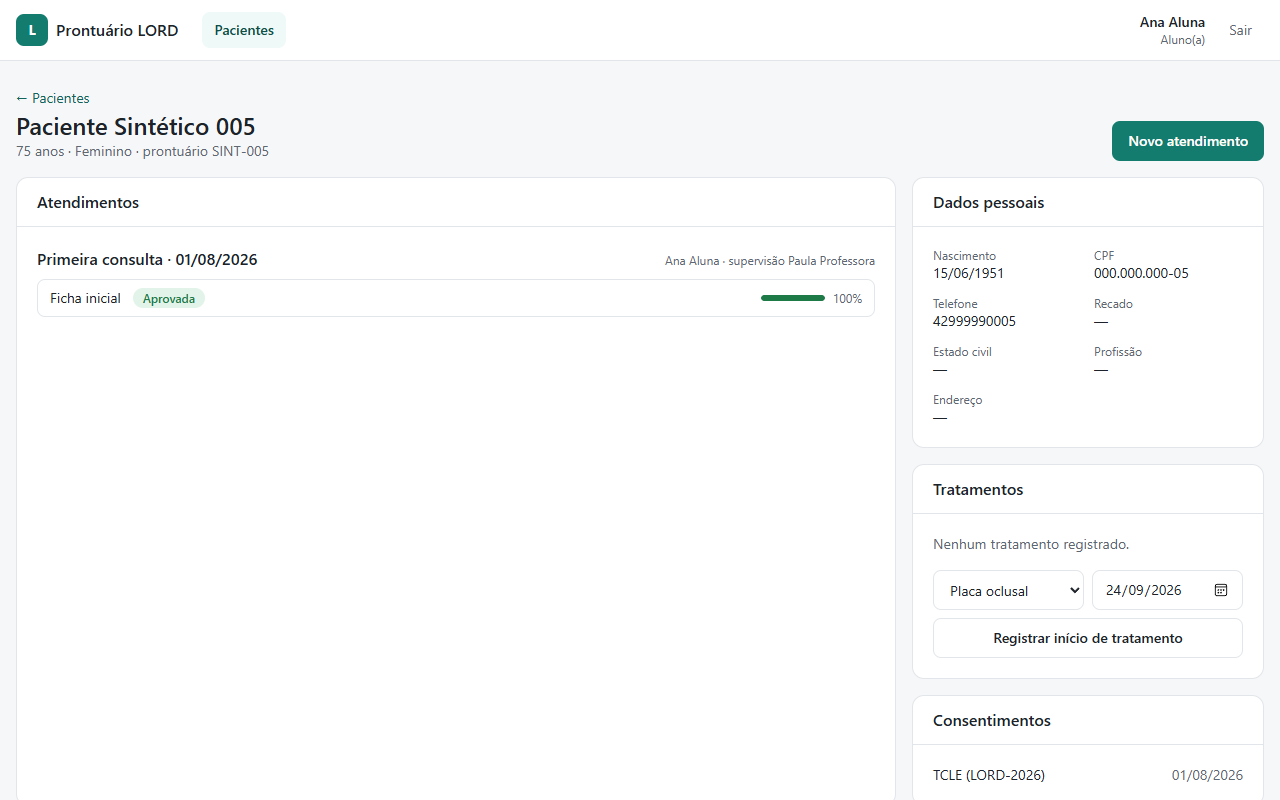
\includegraphics[width=\textwidth]{figuras/03-paciente}
	\fonte{Os autores (2026), com dados sintéticos.}
\end{figure}

O editor da ficha (\autoref{fig:tela-anamnese}) é gerado inteiramente a partir do esquema JSON: cada seção da ficha em papel aparece na navegação lateral com a contagem de campos preenchidos, e cada campo recebe o controle adequado ao seu tipo. Listas de opções viram botões, respostas sim/não viram um par de botões, as escalas de 0 a 10 viram uma régua colorida, e medidas em milímetros viram campos numéricos. O número da questão no papel acompanha cada campo, o que facilita a transição dos alunos habituados à ficha impressa. Campos condicionais, como os medicamentos em uso, só aparecem quando a resposta de controle os torna aplicáveis, e o valor é descartado se a resposta mudar. A validação ocorre no próprio navegador, com o mesmo esquema e as mesmas mensagens usados pela API.

\begin{figure}[htbp]
	\caption{Editor da ficha: seção de história médica}
	\label{fig:tela-anamnese}
	\centering
	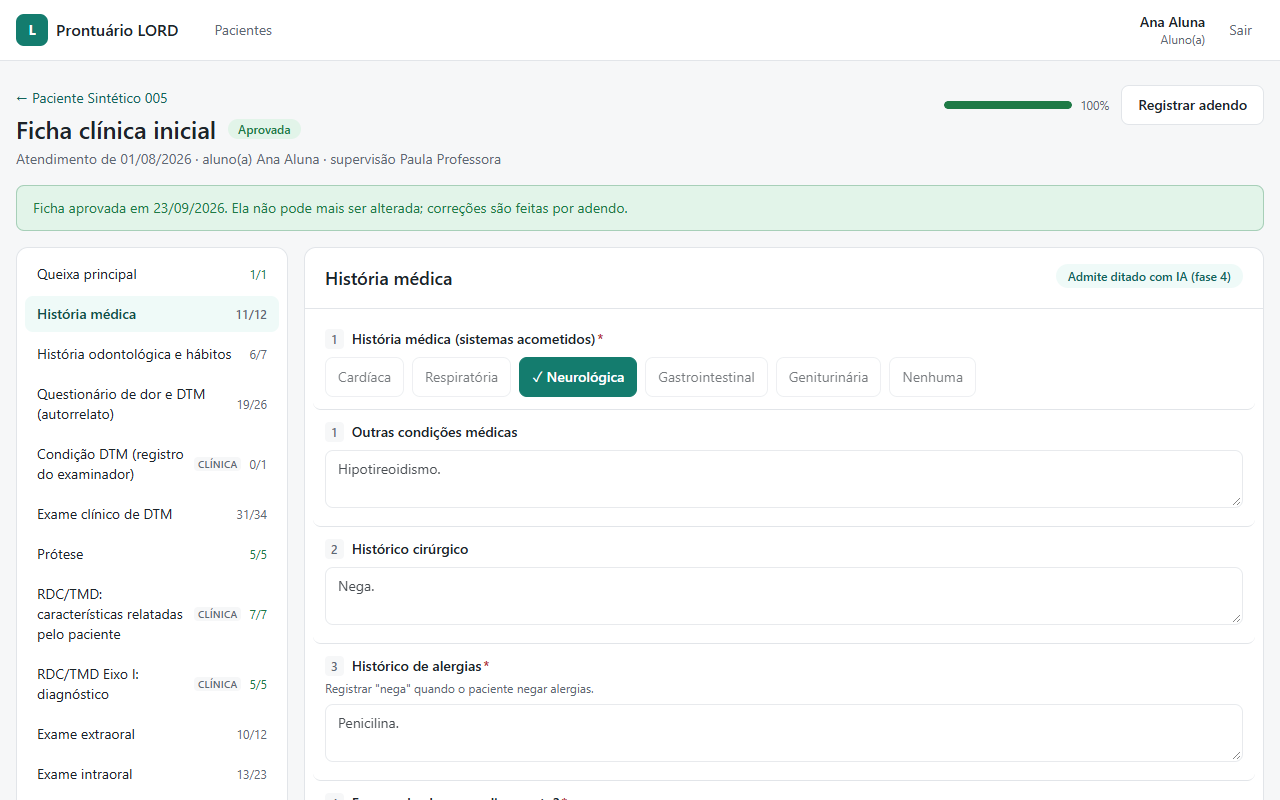
\includegraphics[width=\textwidth]{figuras/04-ficha-historia-medica}
	\fonte{Os autores (2026), com dados sintéticos.}
\end{figure}

A palpação muscular e articular (questões 43 a 45) é registrada em um mapa facial esquemático (\autoref{fig:tela-palpacao}), no qual cada sítio muda de cor conforme a intensidade de 0 a 3. Ao lado há uma tabela equivalente, mais precisa ao toque e acessível por teclado. O odontograma (\autoref{fig:tela-odontograma}) segue a numeração FDI. Cada dente tem cinco faces clicáveis, marcadas segundo a ferramenta escolhida, e a face mesial fica sempre voltada para a linha média. Ao selecionar um dente, é possível registrar sua ausência e condições como tratamento endodôntico ou recessão (RF04).

\begin{figure}[htbp]
	\caption{Mapa de palpação muscular e articular}
	\label{fig:tela-palpacao}
	\centering
	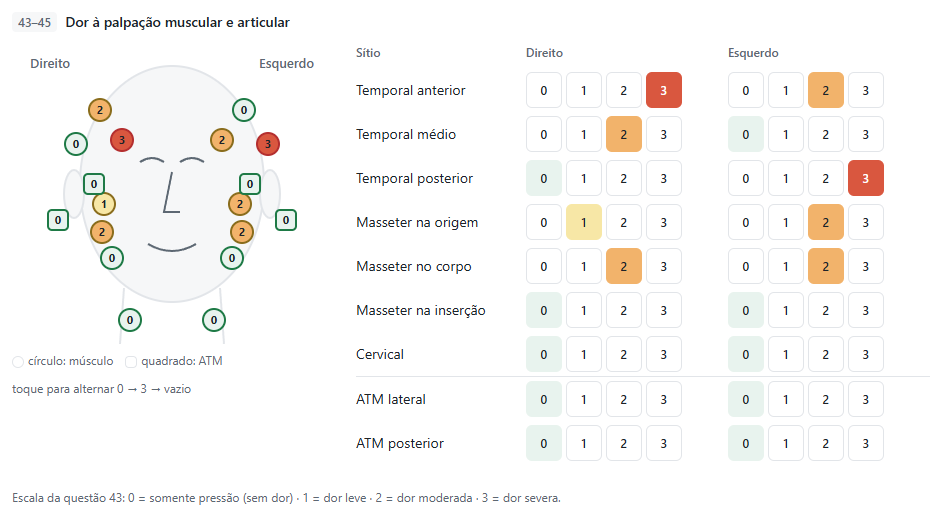
\includegraphics[width=\textwidth]{figuras/06-mapa-palpacao}
	\fonte{Os autores (2026), com dados sintéticos.}
\end{figure}
\begin{figure}[htbp]
	\caption{Odontograma com marcações de exemplo}
	\label{fig:tela-odontograma}
	\centering
	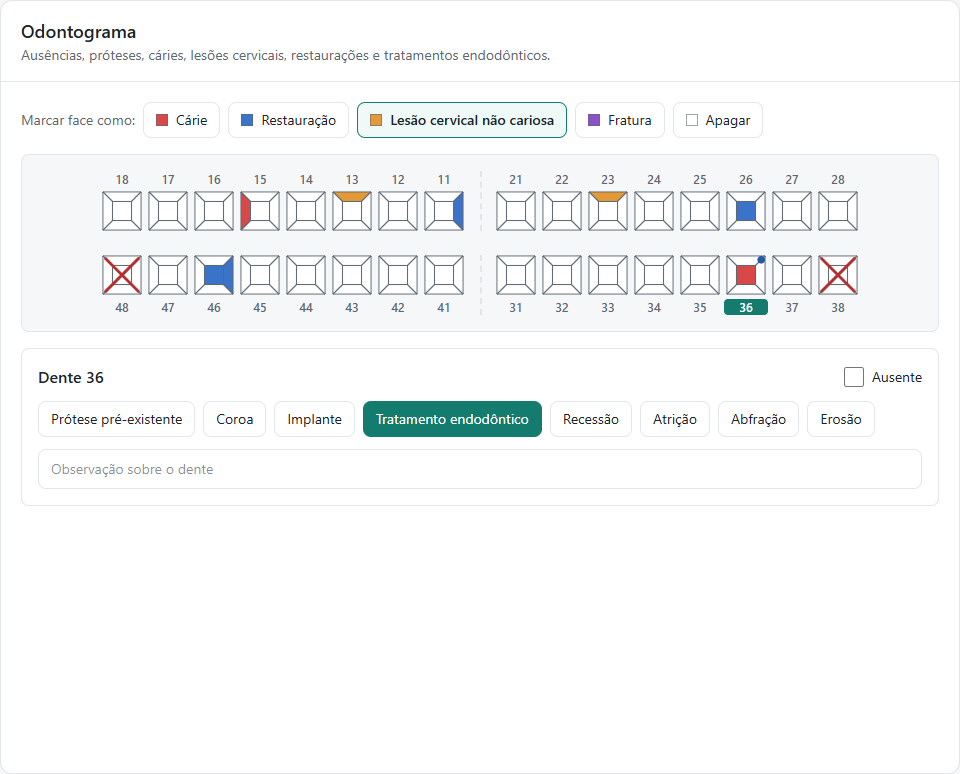
\includegraphics[width=\textwidth]{figuras/08-odontograma}
	\fonte{Os autores (2026), com dados sintéticos.}
\end{figure}

As seções de decisão clínica são identificadas na navegação e no cabeçalho da seção como exclusivas do examinador (\autoref{fig:tela-diagnostico}), reforçando para o usuário a restrição que o esquema impõe ao módulo de IA. O professor acompanha as fichas enviadas pelos alunos em uma fila de revisão (\autoref{fig:tela-revisao}) e, ao abrir cada uma, pode devolvê-la com um comentário ou aprová-la (RF05). Após a aprovação, a ficha é exibida somente para leitura, com a opção de registrar um adendo (RF06).

\begin{figure}[htbp]
	\caption{Seção de diagnóstico, exclusiva do examinador}
	\label{fig:tela-diagnostico}
	\centering
	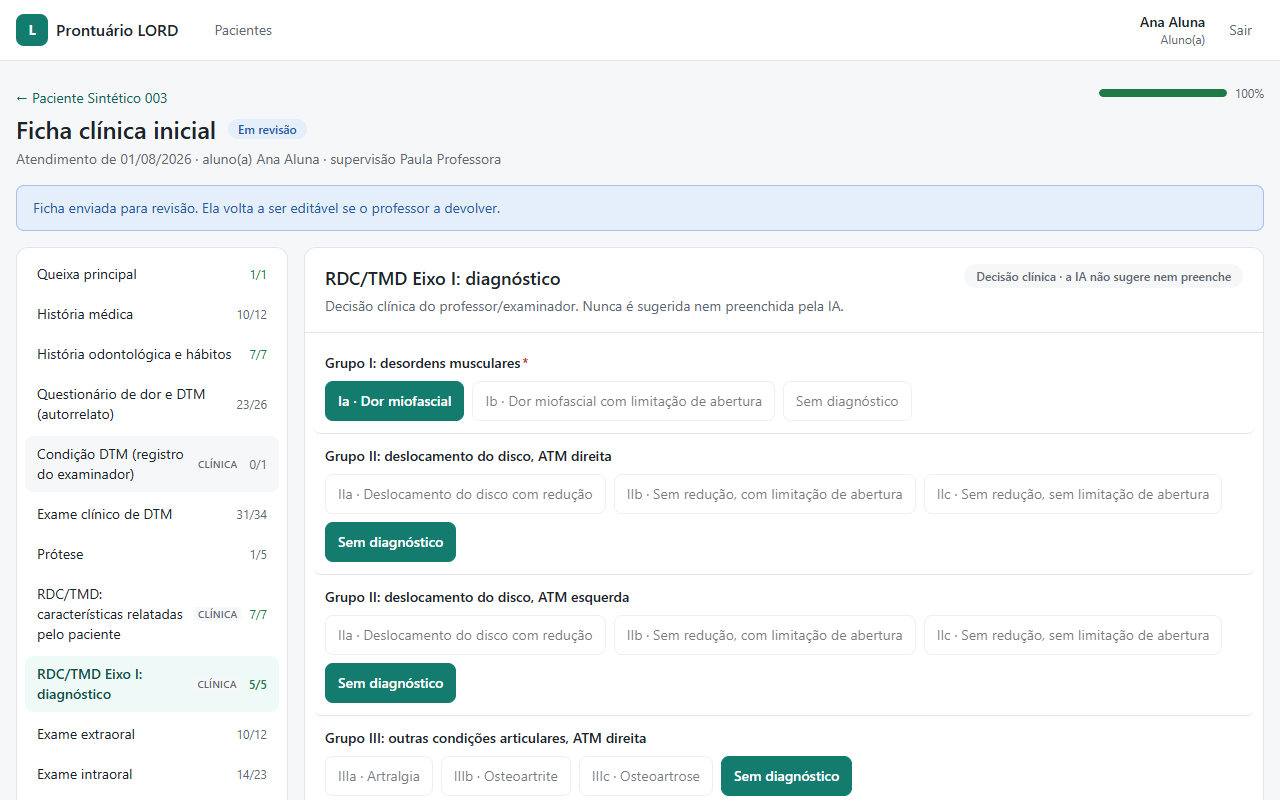
\includegraphics[width=\textwidth]{figuras/07-diagnostico-somente-humano}
	\fonte{Os autores (2026), com dados sintéticos.}
\end{figure}
\begin{figure}[htbp]
	\caption{Fila de revisão do professor}
	\label{fig:tela-revisao}
	\centering
	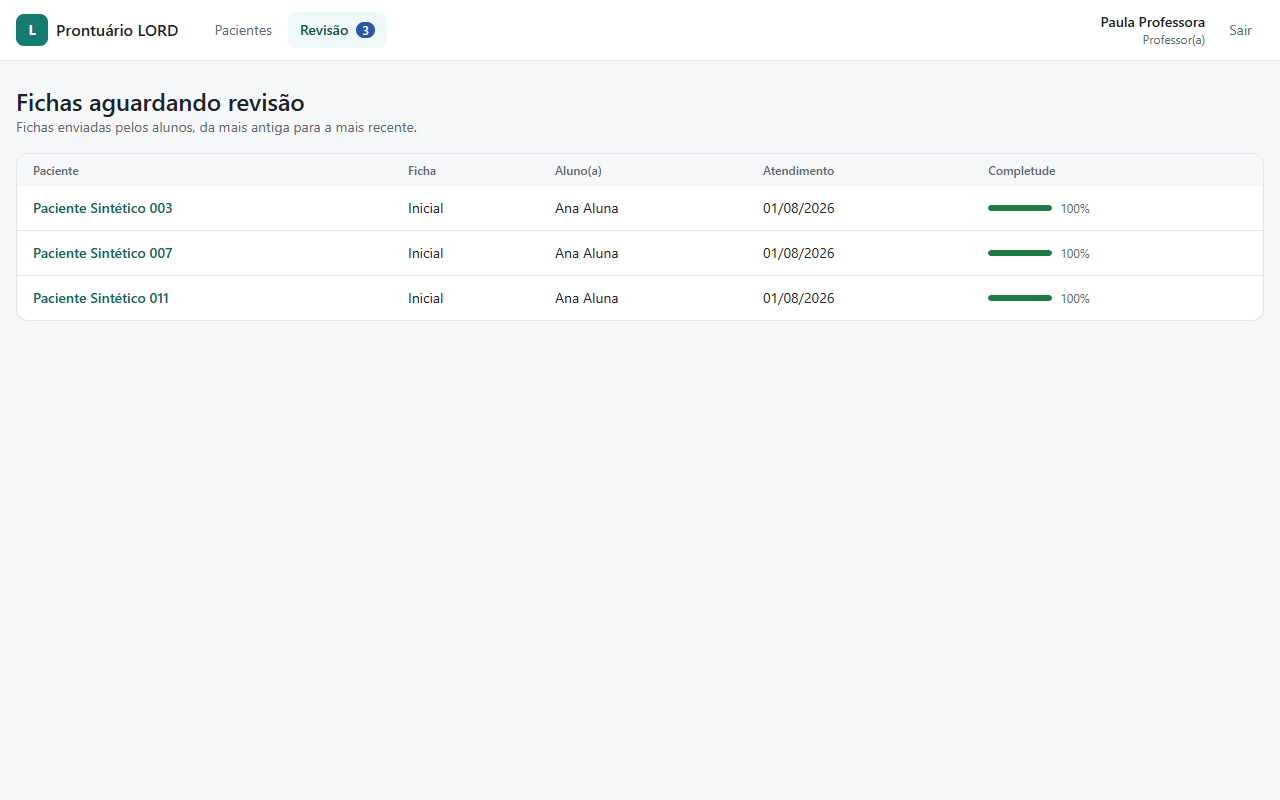
\includegraphics[width=\textwidth]{figuras/09-fila-revisao}
	\fonte{Os autores (2026), com dados sintéticos.}
\end{figure}

Nas seções que admitem ditado, a ficha exibe o painel ``Ditado com IA'' (\autoref{fig:tela-revisao-ia}). O acadêmico grava o relato, que é transcrito e pode ser corrigido antes do envio, ou digita o texto diretamente. As sugestões aparecem com o rótulo do campo, o valor proposto e, entre aspas, o trecho do relato que o justifica. Cada sugestão pode ser aceita ou rejeitada; ao aceitar, o valor é aplicado ao formulário, onde pode ser corrigido, e a decisão passa a constar como ``aceita e editada''. Quando a sugestão substituiria um valor já preenchido, o painel avisa e mostra o valor atual. Os valores descartados pelas salvaguardas ficam em uma lista recolhida, com o motivo do descarte. O painel não aparece nas seções exclusivamente humanas nem em fichas enviadas para revisão ou aprovadas.

\begin{figure}[htbp]
	\caption{Revisão das sugestões da IA com o trecho de evidência}
	\label{fig:tela-revisao-ia}
	\centering
	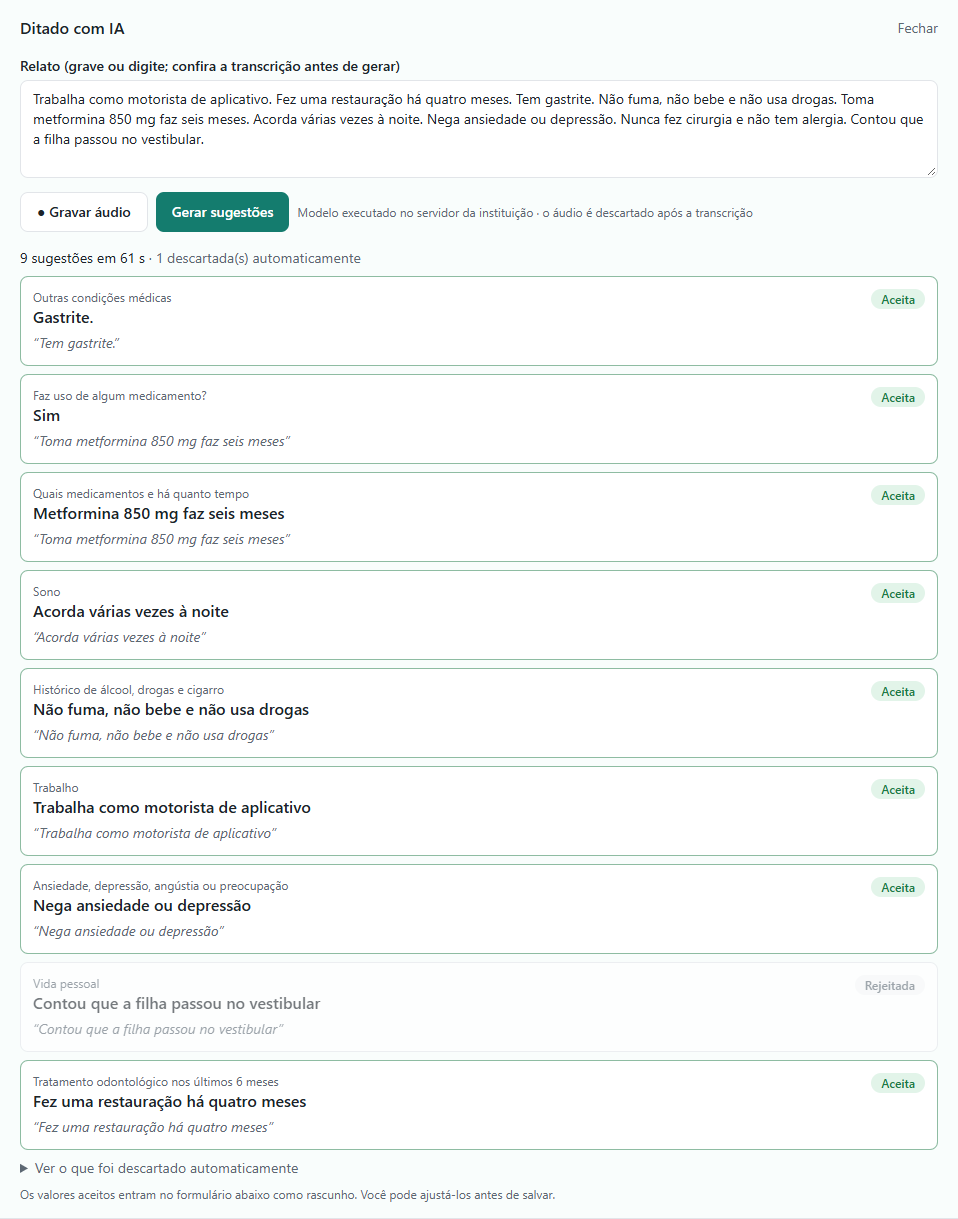
\includegraphics[width=0.85\textwidth]{figuras/11-revisao-ia}
	\fonte{Os autores (2026), com relato sintético e o modelo \texttt{qwen2.5:3b} (\textit{prompt} v4).}
\end{figure}

A \autoref{fig:tela-revisao-ia} foi gerada por um teste automatizado de ponta a ponta que executa o modelo real sobre um relato de desenvolvimento. O relato contém, de propósito, um comentário sem relação com a saúde (``a filha passou no vestibular''). O modelo o atribuiu ao campo ``vida pessoal'', com a citação correta, de modo que as salvaguardas não tinham como barrá-lo. O acadêmico o rejeitou na revisão, o que ilustra por que a revisão humana é obrigatória.

A latência é o principal limite do módulo no ambiente de desenvolvimento, um computador pessoal sem GPU: com o \texttt{qwen2.5:3b}, a estruturação de uma seção isolada pela interface levou de 35 a 104~s, e a das cinco seções que admitem ditado, de 1,3 a 3,8~minutos por relato de desenvolvimento, a uma taxa de cerca de 8~\textit{tokens} por segundo. A transcrição de 14,5~s de áudio pelo Whisper \texttt{small} levou 5,7~s, depois do carregamento inicial do modelo. \todo{medir a latência no servidor da UEPG, com e sem GPU.}

\begin{figure}[htbp]
	\caption{Painel de evolução clínica do paciente}
	\label{fig:tela-painel}
	\centering
	\figtodo{captura do painel do paciente, após a fase 5}
	\fonte{Os autores (2026).}
\end{figure}

\section{Avaliação técnica}

\begin{table}[htbp]
	\caption{Desempenho da persistência híbrida em comparação com o modelo normalizado}
	\label{tb:benchmark}
	\footnotesize
	\centering
	\begin{tabular}{|l|c|c|c|c|}
		\hline
		\multirow{2}{*}{\textbf{Métrica}} & \multicolumn{2}{c|}{\textbf{1.000 pacientes}} & \multicolumn{2}{c|}{\textbf{10.000 pacientes}} \\ \cline{2-5}
		& \textbf{JSONB} & \textbf{Normalizado} & \textbf{JSONB} & \textbf{Normalizado} \\ \hline
		Leitura do prontuário (ms) & -- & -- & -- & -- \\ \hline
		Escrita de um atendimento (ms) & -- & -- & -- & -- \\ \hline
		Espaço em disco (MB) & -- & -- & -- & -- \\ \hline
	\end{tabular}
	\fonte{Os autores (2026).}
\end{table}

Os requisitos de segurança e de integridade são verificados por testes automatizados. Os testes da API são de integração: cada execução cria um servidor PostgreSQL~17 descartável, aplica as migrações e exercita a API por requisições HTTP, verificando também o estado do banco diretamente. Os testes da interface usam a Testing Library para os componentes e o Playwright, com o navegador Microsoft Edge, para os fluxos de ponta a ponta. A \autoref{tb:testes} resume os 142 testes da versão atual. Nos testes do módulo de IA, o modelo de linguagem é substituído por um simulador que devolve respostas preparadas, o que torna os testes rápidos e determinísticos; um teste adicional, executado sob demanda, percorre o fluxo de ditado no navegador com o modelo real.

\begin{table}[htbp]
	\caption{Testes automatizados por componente}
	\label{tb:testes}
	\footnotesize
	\centering
	\begin{tabularx}{\textwidth}{|L{3.8cm}|Y|c|}
		\hline
		\textbf{Componente} & \textbf{O que é verificado} & \textbf{Testes} \\ \hline
		Esquema da ficha & Validade, cobertura das questões 1 a 75, esquema derivado para a IA, rótulos, campos condicionais, completude e salvaguardas da IA (evidência presente no relato, coerência entre valor e evidência, limpeza da citação) & 40 \\ \hline
		API: autenticação & Argon2id, \textit{cookie}, bloqueio, sessão, auditoria de acesso & 9 \\ \hline
		API: controle de acesso & Matriz de papéis na API e \textit{Row-Level Security} diretamente no banco & 10 \\ \hline
		API: pacientes & Cifragem dos dados pessoais, busca por CPF via HMAC, validação, auditoria & 6 \\ \hline
		API: fichas & Fluxo de revisão, imutabilidade, adendos, colunas geradas, odontograma & 7 \\ \hline
		API: esquema analítico & Isolamento do papel analítico, pseudônimos, ausência de textos livres & 5 \\ \hline
		API: sugestões da IA & Recusa de seções exclusivamente humanas e de fichas fora do rascunho, registro das sugestões e das decisões, falha do modelo, auditoria sem conteúdo & 7 \\ \hline
		Módulo de IA & Montagem do \textit{prompt}, formato de saída, descarte pelas salvaguardas (com modelo simulado), métricas e retomada do Experimento~A, distinção entre falha de conexão e saída inválida & 14 \\ \hline
		Serviço de transcrição & Idioma e vocabulário clínico enviados ao modelo, áudio mantido só em memória, recusa de arquivos que não são áudio, vazios, grandes demais ou ilegíveis & 6 \\ \hline
		Interface: componentes & Controle por tipo de campo, campos condicionais, erros, mapa de palpação, odontograma e painel de ditado (aceitar, rejeitar, aceitar todas, edição posterior) & 24 \\ \hline
		Interface: ponta a ponta & Fluxo completo da ficha no navegador (cadastro, preenchimento, persistência, revisão, aprovação) e restrição de telas por papel & 2 \\ \hline
		Gerador de casos sintéticos & Validade, reprodutibilidade, coerência clínica e compatibilidade com o sexo & 12 \\ \hline
		\textbf{Total} & & \textbf{142} \\ \hline
	\end{tabularx}
	\fonte{Os autores (2026).}
\end{table}

Entre as propriedades verificadas estão as seguintes. Um aluno não obtém, nem pela API nem por consulta direta com o papel da aplicação, os pacientes de outro aluno. O administrador não enxerga pacientes, embora consulte a auditoria. Nem o dono das tabelas consegue alterar ou excluir uma ficha aprovada. O texto original do CPF, do telefone e do endereço não aparece no valor gravado. O papel analítico não tem acesso às tabelas identificadas nem ao segredo dos pseudônimos, e as visões analíticas não contêm o nome do paciente nem trechos de texto livre.

\todo{resultado da varredura OWASP ZAP (alertas por severidade, antes e depois) e cobertura de testes.}

\section{Experimento A: qualidade da estruturação automática}

\begin{table}[htbp]
	\caption{Desempenho da estruturação automática no conjunto de teste}
	\label{tb:exp-a}
	\footnotesize
	\centering
	\begin{tabular}{|l|l|c|c|c|c|c|c|}
		\hline
		\textbf{Modelo} & \textbf{Estratégia} & \textbf{P} & \textbf{R} & \textbf{F1} & \textbf{Alucinação} & \textbf{Omissão} & \textbf{Latência (s)} \\ \hline
		Modelo 1 & Ficha inteira & -- & -- & -- & -- & -- & -- \\ \hline
		Modelo 1 & Por seção & -- & -- & -- & -- & -- & -- \\ \hline
		Modelo 2 & Ficha inteira & -- & -- & -- & -- & -- & -- \\ \hline
		Modelo 2 & Por seção & -- & -- & -- & -- & -- & -- \\ \hline
	\end{tabular}
	\fonte{Os autores (2026).}
\end{table}

\todo{F1 por seção da ficha (gráfico), validade estrutural, reprodutibilidade e análise qualitativa dos erros por categoria: negação, tempo, autocorreção, termos coloquiais.}

\section{Experimento B: captação por áudio versus texto}

\begin{table}[htbp]
	\caption{Taxa de erro de palavras e impacto na estruturação}
	\label{tb:exp-b}
	\footnotesize
	\centering
	\begin{tabular}{|l|l|c|c|c|}
		\hline
		\textbf{Modelo Whisper} & \textbf{Condição} & \textbf{WER geral} & \textbf{WER termos clínicos} & \textbf{$\Delta F_1$ vs. texto} \\ \hline
		\textit{small} & Silêncio & -- & -- & -- \\ \hline
		\textit{small} & Ruído & -- & -- & -- \\ \hline
		\textit{medium} & Silêncio & -- & -- & -- \\ \hline
		\textit{medium} & Ruído & -- & -- & -- \\ \hline
	\end{tabular}
	\fonte{Os autores (2026).}
\end{table}

\section{Experimento C: usabilidade e eficiência}

\todo{caracterização dos participantes (número, período do curso, experiência com a ficha).}

\begin{table}[htbp]
	\caption{Resultados por condição de registro}
	\label{tb:exp-c}
	\footnotesize
	\centering
	\begin{tabular}{|l|c|c|c|c|}
		\hline
		\textbf{Condição} & \textbf{Tempo (min)} & \textbf{Completude (\%)} & \textbf{Erros} & \textbf{NASA-TLX} \\ \hline
		Papel & -- & -- & -- & -- \\ \hline
		Formulário digital & -- & -- & -- & -- \\ \hline
		Formulário com ditado e IA & -- & -- & -- & -- \\ \hline
	\end{tabular}
	\fonte{Os autores (2026).}
\end{table}

\todo{escore SUS médio e intervalo de confiança; resultado do teste de Friedman; taxa de aceitação das sugestões; problemas de usabilidade por severidade; síntese das entrevistas.}

\section{Experimento D: validação do pipeline analítico}

\begin{table}[htbp]
	\caption{Efeitos programados e efeitos recuperados na coorte sintética}
	\label{tb:exp-d}
	\footnotesize
	\centering
	\begin{tabular}{|l|c|c|c|c|}
		\hline
		\textbf{Tratamento} & \textbf{Redução programada} & \textbf{Redução estimada} & \textbf{$p$ (Wilcoxon)} & \textbf{Redução $\geq$ 30\%} \\ \hline
		Placa oclusal & 40\% & -- & -- & -- \\ \hline
		Orientações & 10\% & -- & -- & -- \\ \hline
	\end{tabular}
	\fonte{Os autores (2026).}
\end{table}

\begin{figure}[htbp]
	\caption{Painel de coorte gerado a partir da coorte sintética}
	\label{fig:painel-coorte}
	\centering
	\figtodo{diagramas de caixa da variação da dor por tratamento e prevalência das características relatadas}
	\fonte{Os autores (2026).}
\end{figure}

	\chapter{Discussão}
\label{cap:discussao}

\todo{discutir os resultados à luz das três questões que orientaram o projeto, comparando com a literatura do Capítulo~\ref{cap:trabalhos}.}

\section{Onde armazenar os dados}

\todo{discutir a execução integral em infraestrutura institucional: custo, desempenho observado dos modelos locais sem GPU e implicações para a LGPD.}

\section{IA sem finalidade diagnóstica}

\todo{discutir a taxa de alucinação e a de aceitação das sugestões, o papel do trecho de evidência e a eficácia das salvaguardas.}

\section{Áudio ou formulário}

\todo{discutir, com base nos Experimentos B e C, em que partes da ficha o ditado compensa e em quais o formulário é superior.}

\section{Limitações}
\label{sec:limitacoes}

\begin{itemize}
	\item \textbf{Dados sintéticos}: os experimentos de IA e de análise utilizam casos e coortes fictícios. Eles demonstram o funcionamento dos módulos, mas não permitem conclusões clínicas sobre a eficácia dos tratamentos da Liga. Narrativas redigidas a partir de gabaritos podem ser mais organizadas que consultas reais.
	\item \textbf{Amostra da avaliação de usabilidade}: o número reduzido de participantes, todos de uma mesma Liga, limita a generalização dos resultados quantitativos.
	\item \textbf{Instrumento clínico}: a ficha da Liga baseia-se no RDC/TMD \cite{dworkin1992}, já sucedido pelo DC/TMD \cite{schiffman2014}. O esquema versionado permite a migração, mas ela não foi realizada neste trabalho.
	\item \textbf{Validade legal}: sem assinatura digital com certificação ICP-Brasil, o sistema não substitui o prontuário em papel \cite{cfo91-2009}.
	\item \textbf{Interoperabilidade}: o sistema não troca dados com outros sistemas de saúde, como a Rede Nacional de Dados em Saúde, nem adota padrões como o HL7 FHIR.
	\item \textbf{Escalabilidade}: a implantação prevê um único servidor, adequado ao volume da Liga, mas não a uma clínica-escola inteira sem ajustes de infraestrutura.
	\item \textbf{Desempenho da IA}: sem GPU, o tempo de resposta dos modelos locais pode ser elevado; modelos menores são mais rápidos, porém menos precisos.
	\item \textbf{Vieses dos modelos}: modelos de fala e de linguagem podem ter desempenho inferior com sotaques regionais, fala espontânea e vocabulário muito específico.
\end{itemize}
    % Discussão e limitações
	\chapter{Conclusão}
\label{cap:conclusao}

A digitalização direcionada e arquitetada especificamente para o acompanhamento odontológico contínuo mostrou-se um caminho promissor. A proposta não se resume a evitar a perda física de papéis: trata-se de introduzir uma cultura analítica, orientada a dados, no ambiente de ensino e prática clínica da UEPG, sem transferir à máquina a responsabilidade pelo diagnóstico.

\todo{retomar cada objetivo específico e indicar como foi atingido, com os principais números dos experimentos.}

\section{Trabalhos futuros}

\begin{itemize}
	\item Implantação em atendimentos reais após aprovação ética e adoção de termo de consentimento para gravação de áudio;
	\item Assinatura digital com certificação ICP-Brasil, permitindo a eliminação do prontuário em papel;
	\item Migração da ficha para o DC/TMD, aproveitando o esquema versionado;
	\item Preenchimento do questionário de autorrelato pelo próprio paciente em \textit{tablet}, na sala de espera;
	\item Interoperabilidade com a Rede Nacional de Dados em Saúde por meio do padrão HL7 FHIR;
	\item Ampliação para outras ligas e clínicas do curso de Odontologia da UEPG.
\end{itemize}

	
	\postextual
	%ljsenger - espaçamento entre o título e o primeiro parágrafo do texto
	\setlength\afterchapskip{18pt}
	%ljsenger - adeus a caixa alta
	\bibliographystyle{tcc-uepg}
	\bibliography{base}

% ----------------------------------------------------------
% Glossário
% ----------------------------------------------------------
%
% Consulte o manual da classe abntex2 para orientações sobre o glossário.
%
%\glossary

% ----------------------------------------------------------
% Apêndices
% ----------------------------------------------------------

% ---
% Inicia os apêndices
% ---
\begin{apendicesenv}

	\renewcommand{\thetable}{\Alph{chapter}\arabic{table}}
	\setcounter{table}{0}

	% ---------------------------------------------------------------------
\chapter{Trecho do esquema JSON da ficha clínica}
\label{apendice:schema}

O esquema completo está no repositório do sistema, em \texttt{packages/ficha/schemas}. O \autoref{cod:schema} mostra parte de três seções da ficha inicial. A seção de história médica admite ditado. O questionário de dor admite apenas formulário, de modo que a IA não atribui notas de dor. O diagnóstico do Eixo~I é exclusivamente humano. As definições reutilizáveis, como a escala de 0 a 10, ficam no esquema comum e são referenciadas por \texttt{\$ref}.

\begin{lstlisting}[caption={Trecho do esquema da ficha inicial (versão 1)}, label=cod:schema]
{
  "$id": "urn:lord-uepg:ficha-inicial:v1",
  "type": "object",
  "additionalProperties": false,
  "properties": {
    "historia_medica": {
      "x-captacao": ["ditado", "formulario"],
      "type": "object",
      "additionalProperties": false,
      "properties": {
        "q3_alergias": {
          "title": "Histórico de alergias",
          "x-questao": "3",
          "x-obrigatorio": true,
          "$ref": "urn:lord-uepg:comum:v1#/$defs/texto"
        },
        "q4_usa_medicamento": {
          "title": "Faz uso de algum medicamento?",
          "x-questao": "4",
          "$ref": "urn:lord-uepg:comum:v1#/$defs/simNao"
        }
      }
    },
    "questionario_dtm": {
      "x-captacao": ["formulario"],
      "properties": {
        "q16_dor_atual": {
          "title": "Nota da dor na face neste momento (0 a 10)",
          "x-questao": "16",
          "$ref": "urn:lord-uepg:comum:v1#/$defs/escala0a10"
        }
      }
    },
    "diagnostico_eixo1": {
      "x-somente-humano": true,
      "properties": {
        "grupo1_muscular": {
          "enum": ["Ia_dor_miofascial",
                   "Ib_dor_miofascial_com_limitacao_abertura",
                   "sem_diagnostico", null]
        }
      }
    }
  }
}
\end{lstlisting}

O \autoref{cod:schema-ia} mostra o esquema derivado automaticamente para um campo da história médica, que é o formato enviado ao modelo de linguagem. A derivação resolve as referências, remove os metadados, mantém as instruções de preenchimento do próprio campo e exige, para cada campo, o valor e o trecho da transcrição que o justifica.

\begin{lstlisting}[caption={Esquema derivado para a IA (campo de alergias)}, label=cod:schema-ia]
"q3_alergias": {
  "type": "object",
  "additionalProperties": false,
  "description": "Histórico de alergias",
  "properties": {
    "valor": {
      "type": ["string", "null"],
      "maxLength": 4000,
      "description": "Registrar \"nega\" quando o paciente negar alergias."
    },
    "evidencia": {
      "type": ["string", "null"],
      "description": "Trecho literal da transcrição que justifica
                      o valor; null se não mencionado."
    }
  },
  "required": ["valor", "evidencia"]
}
\end{lstlisting}

% ---------------------------------------------------------------------
\chapter{Roteiro da avaliação de usabilidade}
\label{apendice:usabilidade}

\section{Tarefas}

\begin{enumerate}
	\item Acessar o sistema com o usuário de teste;
	\item Cadastrar o paciente do caso simulado;
	\item Registrar a anamnese e o exame clínico na condição sorteada (papel, formulário digital ou formulário com ditado e IA);
	\item Enviar a ficha para revisão;
	\item (Professores) Revisar, devolver com comentário e aprovar uma ficha.
\end{enumerate}

\section{Questionário SUS}

Cada item é respondido em escala de 1 (discordo totalmente) a 5 (concordo totalmente). O escore é obtido subtraindo 1 das respostas dos itens ímpares e subtraindo de 5 as respostas dos itens pares; a soma é multiplicada por 2,5, resultando em um valor de 0 a 100 \cite{brooke1996}.

\begin{enumerate}
	\item Eu acho que gostaria de usar este sistema com frequência.
	\item Eu achei o sistema desnecessariamente complexo.
	\item Eu achei o sistema fácil de usar.
	\item Eu acho que precisaria do apoio de um técnico para conseguir usar este sistema.
	\item Eu achei que as diversas funções deste sistema estavam bem integradas.
	\item Eu achei que havia muita inconsistência neste sistema.
	\item Eu imagino que a maioria das pessoas aprenderia a usar este sistema rapidamente.
	\item Eu achei o sistema muito complicado de usar.
	\item Eu me senti muito confiante usando o sistema.
	\item Eu precisei aprender muitas coisas antes de conseguir usar este sistema.
\end{enumerate}

\todo{substituir por uma tradução validada do SUS para o português e citar a fonte.}

\section{Entrevista semiestruturada}

\begin{enumerate}
	\item O que foi mais fácil e o que foi mais difícil em cada forma de registro?
	\item Você confiou nas sugestões da IA? Em que situações precisou corrigi-las?
	\item Em que momentos do atendimento você usaria o ditado? Em quais não usaria?
	\item O que falta no sistema para substituir a ficha em papel na rotina da Liga?
\end{enumerate}

% ---------------------------------------------------------------------
\chapter{Matriz de controle de acesso}
\label{apendice:rbac}

\begin{table}[htbp]
	\caption{Permissões por papel}
	\label{tb:rbac}
	\footnotesize
	\centering
	\begin{tabular}{|l|c|c|c|c|}
		\hline
		\textbf{Ação} & \textbf{Aluno} & \textbf{Professor} & \textbf{Pesquisador} & \textbf{Administrador} \\ \hline
		Cadastrar paciente & Sim & Sim & Não & Não \\ \hline
		Ver prontuário identificado & Próprios & Sim & Não & Não \\ \hline
		Preencher ficha (rascunho) & Sim & Sim & Não & Não \\ \hline
		Usar ditado e IA & Sim & Sim & Não & Não \\ \hline
		Aprovar ficha & Não & Sim & Não & Não \\ \hline
		Registrar adendo em ficha aprovada & Sim & Sim & Não & Não \\ \hline
		Ver painel do paciente & Próprios & Sim & Não & Não \\ \hline
		Ver painéis de coorte & Não & Sim & Sim & Não \\ \hline
		Exportar dados pseudonimizados & Não & Não & Sim & Não \\ \hline
		Gerenciar usuários & Não & Não & Não & Sim \\ \hline
		Consultar auditoria & Não & Não & Não & Sim \\ \hline
	\end{tabular}
	\fonte{Os autores (2026).}
\end{table}

\todo{confirmar a matriz com a coordenação da LORD.}


\end{apendicesenv}
% ---


% ----------------------------------------------------------
% Anexos
% ----------------------------------------------------------
\begin{anexosenv}

	\chapter{Ficha clínica da LORD-UEPG}
	\label{anexo:ficha}
	Ficha clínica em papel utilizada pela Liga Odontológica de Reabilitação e DTM (LORD-UEPG), incluindo o Termo de Consentimento Livre e Esclarecido, reproduzida sem dados de pacientes. Ela é a fonte dos requisitos de dados do sistema (\autoref{sec:ficha}).

	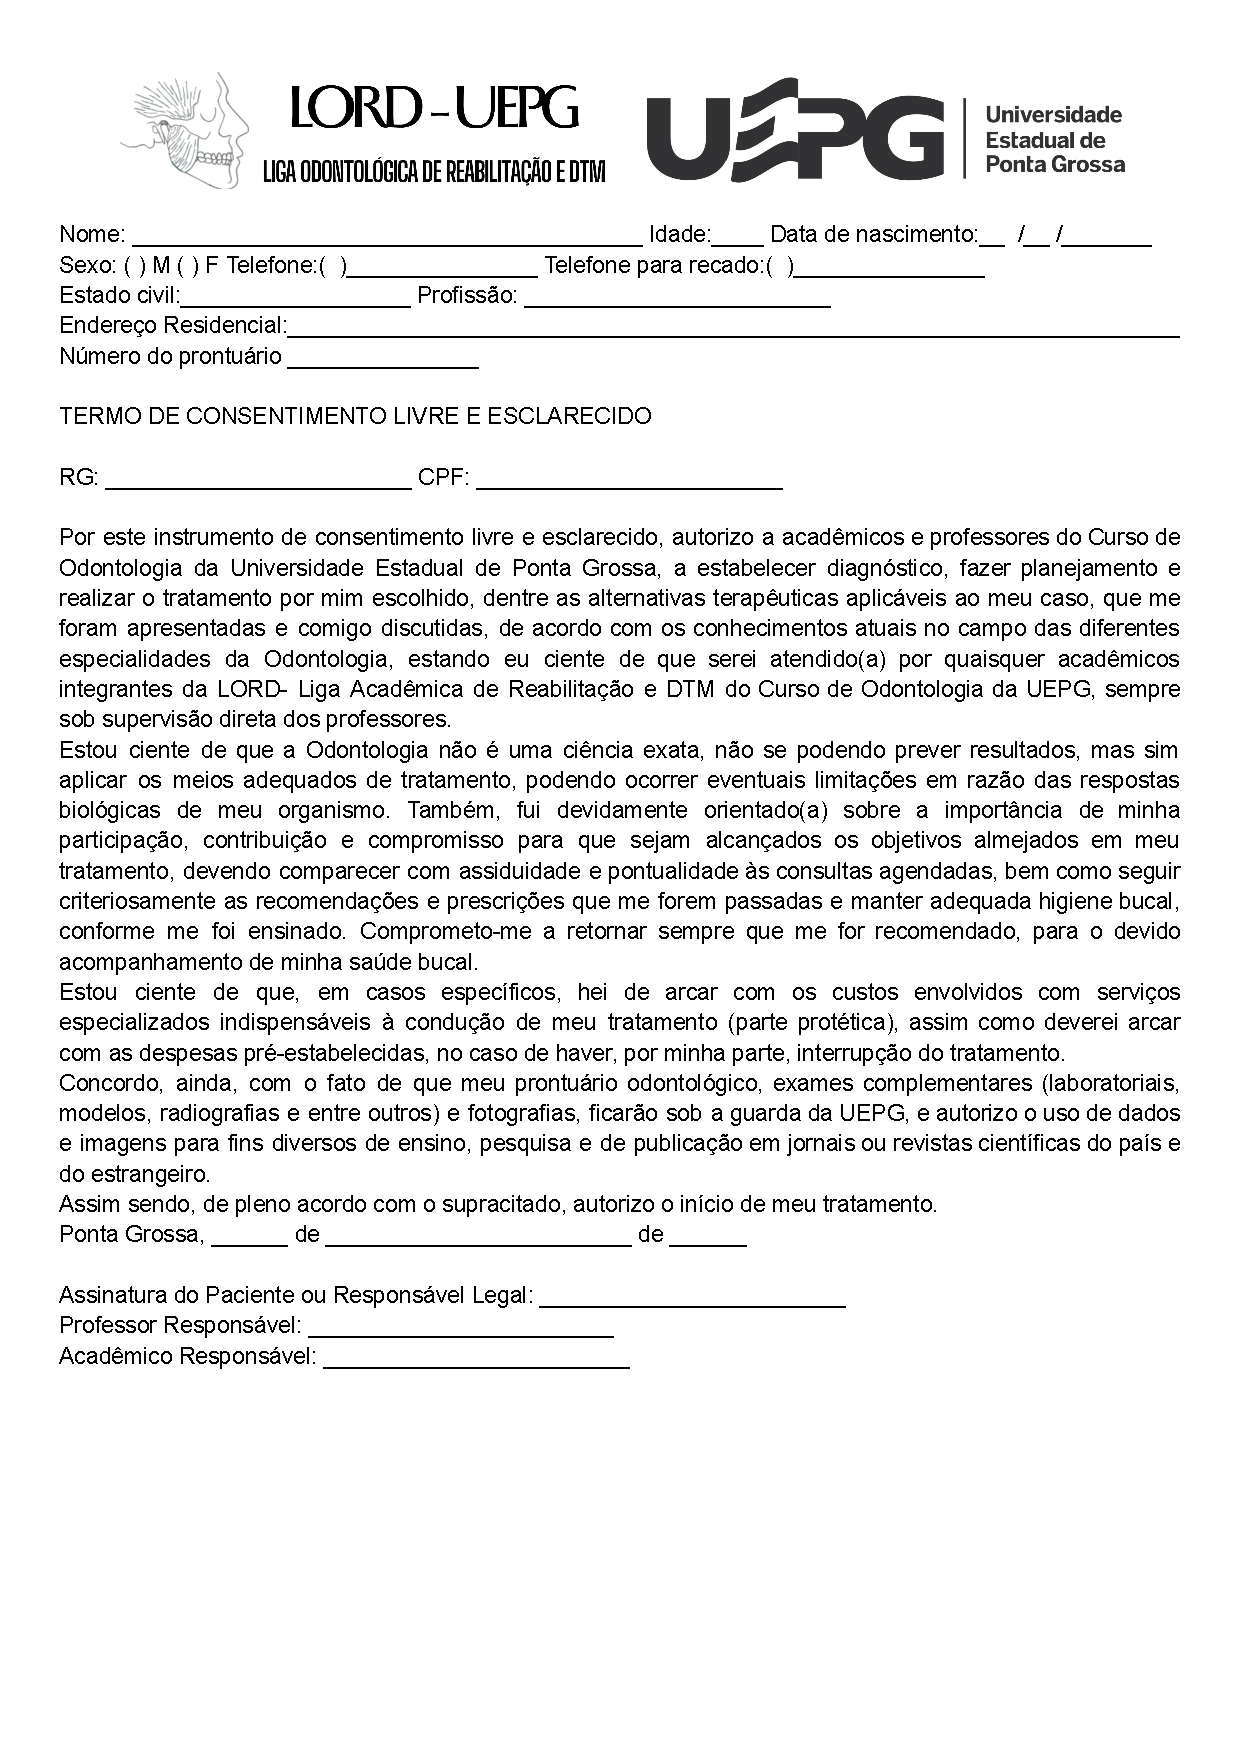
\includepdf[pages=-,scale=0.85,pagecommand={}]{ficha-lord}

\end{anexosenv}

%---------------------------------------------------------------------
% INDICE REMISSIVO
%---------------------------------------------------------------------
\phantompart
\printindex
%---------------------------------------------------------------------

\end{document}	
